\documentclass[a4paper,12pt]{article}
\usepackage{array}
\usepackage{listings}
\usepackage{graphicx}
\graphicspath{ {./images/} }

\setlength{\tabcolsep}{18pt}
\renewcommand{\arraystretch}{1.2}


\begin{document}
\title{Zusammenfassung Informationssicherheit}
\author{Mathis Hermann}
\date{\today}
\maketitle

Diese Zusammenfassung ist basierend auf den gegebenen Unterlagen. Alle Angaben ohne Gewähr. Weitergabe und Verbreitung erlaubt nur mit expliziter Genehmigung.

\section{Gesetzliche Grundlagen}
Schweizer Recht ist uneingeschränkt anwendbar, wenn Täter, Opfer und Tatort in der Schweiz liegen. Im Internet ist das ein Problem.

\subsection{Gesetzestexte}
Es gibt keum für das Internet spezifische Gesetzestexte in der Schweiz. Es gibt aber viele Gesetzestexte, die im Zusammenhang mit dem Internet angewendet werden: \emph{1)} Obligationenrecht, \emph{2)} Strafgesetzbuch,  \emph{3)} Datenschutzgesetz,  \emph{4)} Fernmeldegesetz,  \emph{5)} Urheberrechtsgesetz -- (Liste nicht abschliessend)

Dabei können auch diverse Unterschiede zwischen CH und EU-Recht gefunden werden.
\begin{center}
\begin{tabular}{ | m{2.5cm} | m{4.5cm} | m{4.5cm} | } 
Recht & CH & EU\\ 
\hline
Widerrufsrecht & Freiwillig (10 Tage) & 14 Tage\\
Lieferfrist & Keine Obergrenze & maximal 30 Tage; länger kann verabredet werden\\
Gewährleistung & 2 Jahre & 2 Jahre\\
Bestell-Button & Keine Vorgabe & Muss als letzter Punkt des "Vertrages" auf der Seite stehen und mit "Zahlungspflichtig bestellen" \emph{eindeutig} beschriftet sein.\\
Preise & Tatsächlich zu bezahlender Preis in CHF inkl. aller nicht frei wählbarer Zuschläge jeglicher Art. Einheiten und Verrechnungssätze müssen klar ersichtlich sein. & Gesamtpreis einschliesslich aller Steuern und Abgaben.\\
\end{tabular}
\end{center}




\paragraph{Obligationenrecht} Definiert Formvorschrift: Es braucht im Allgemeinen keine besondere Form für das Zustandekommen eines Vertrages.

Alle Parteien haben Rechte und Pflichten:
\begin{itemize}
\item Vertrag muss eingehalten werden
\item Haftbarkeit bei versäumten Pflichten
\item Kein Recht ohne Verpflichtungen
\end{itemize}



\paragraph{Datenschutzgesetz}  Gilt für das Bearbeiten von Daten natürlicher und juristischer Personen. Informationen können mit Verweis auf Datenschutz Gericht nicht vorenthalten werden.

\begin{itemize}
\item Personendaten -- alle Angaben, die sich auf eine bestimmte oder bestimmbare Person beziehen
\item Betroffene Personen -- natürliche oder juristische Personen, über die Daten bearbeitet werden
\item Besonders Schützenswerte Personendaten -- Daten über:
    \begin{itemize}
    \item die religiösen, weltanschaulichen, politischen, oder gewerkschaftlichen Ansichten oder Tätigkeiten
    \item die Gesundheit, Intimsphäre oder Rassenzugehörigkeit
    \item Massnahmen der sozialen Hilfe
    \item Administrative oder strafrechtliche Verfolgungen und Sanktionen
    \end{itemize}
\end{itemize}

Jede Person kann vom Inhaber einer Datensammlung Auskunft darüber verlangen, ob Daten über sie bearbeitet werden. Lässt der Inhaber der Datensammlung Personendaten durch einen Dritten bearbeiten, so bleibt er auskunftspflichtig. Die Auskunft ist in der Regel schriftlich, in Form eines Ausdrucks oder einer Fotokopie sowie kostenlos zu erteilen.


\paragraph{Fernmeldegesetz} Es ist eine Meldeplficht für Fernmeldeanlagen definiert -- \emph{Fernmeldedienst}: fernmeldetechnische Übertragung von Informationen für Dritte; Senden und Empfangen von Informationen über Leitungen oder Funk etc.

WLAN-Accesspoint, Mailserver, Chatserver Gameserver mit Chatfunktion, Powerline-LAN sind grundsätzlich meldepflichtig -- Paragraph 2 bestimmt Ausnahmen.

\paragraph{Urheberrechtsgesetz} Werke sind, unabhängig von ihrem Wert pder Zweck, geistige Schöpfungen der Literatur und Kunst, die individuellen Charakter haben. Urheber:in ist Person, welche das Werk geschaffen hat. Urheber:in hat das auschliessliche Recht über das zu bestimmen, ob, wann und wie das Werk verwendet wird.

Wird in einem Arbeitsverhältnis bei Ausübung dienstlicher Tätigkeiten sowie in \emph{Erfüllung vertraglicher Pflichten} ein Computerprogramm geschaffen, so ist Arbeitgeber:in allein zur Ausübung der ausschliesslichen Verwendungsbefugnisse berechtigt.

\subsection{revDSG}
Per Juni 2023 wird eine Revision des Datenschutzgesetzes eingeführt:
\begin{itemize}
\item Nur noch natürliche Personen sind geschützt
\item Genetische und biometrische Daten werden besonders schützenswerte Daten
\item Grundsätze "Privacy by Design" und "Privacy by Default" werden eingeführt
\item Informationspflicht gilt für jede From von Personendaten
\item Ein Verzeichnis der Bearbeitungstätigkeiten wird zur Pflicht
\item Pflicht zur raschen Meldung bei Verletzung der Datensicherheit
\end{itemize}

\subsection{Praxis}

\paragraph{Impressumspflicht} gilt typischerweise sobald eine Website gewerblich oder kommerziell ist. Impressum muss leicht auffindbar sein und Vorname und Name (bzw. Firma), Adresse und E-Mail-Adressen beinhalten.

\paragraph{Abschliessend} Informatiker:innen unterliegen beim Schreiben eines Programmes oder Aufsetzen eines Servers im Minimum immer der schweizerischen Gesetzgebung. Es existieren viele Gesetze, welche einfach zu übertreten sind, aber nicht übertreten werden dürfen.

Im Internet müssen je nachdem auch Gesetze von Drittstaaten berücksichtigt werden.

Gesetzestexte wurden nicht für Laien und nicht von technischen Fachleuten geschrieben. Gesetzestexte folgen nicht immer der Vernunft oder Logik.

Publikationen können helfen Zweifelsfälle zu beantworten.






\newpage
\section{Sicherheitsvokabular}

\subsection{Das Sicherheitsvokabular}

\begin{itemize}
\item \emph{Confidentiality / Vertraulichkeit} -- gewährleistet, dass Daten nur für befugte Entitäten zugänglich sind.
\item \emph{Integrity / Integrität} -- gewährleistet, dass Daten, Programme oder Funktionen in unveränderter Form belassen werden (immer gemessen am Sollzustand).
\item \emph{Availabtility / Verfügbarkeit} -- gewährleistet, dass eine Funktion immer dem Funktionsbezüger zur Verfügung steht.
\item \emph{Authenticity / Authentizität} -- Echtheit, Überprüfbarkeit, Vertrauenswürdigkeit eines Objektes.
\item \emph{Non-Repudiation / Nicht-Abstreitbarkeit} -- Es kann nachgewiesen werden, dass eine Handlung tatsächlich stattgefunden hat.
\item \emph{Accountability / Verbindlichkeit} -- Konsequenzen einer Handlung sind rechtlich bindend.
\item \emph{Asset / Aktivposten} -- Mit einem Aktivposten wird Wert verbunden; ist meistens subjektiv
\item \emph{Threat / Bedrohung} -- mögliche Gefahr, die eines der Assets in seinen Schutzzielen beeinträchtigen könnte
\item \emph{Vulnerability / Schwäche} -- Zustand oder Begebenheit, durch die ein Asset gefährdet sein könnte
\item \emph{Single Loss Expectancy / Schadensausmass} -- Wert, der die Höhe des einzelnen Schadensereigneisses bemisst
\item \emph{Probability of Occurence / Eintrittswahrscheinlichkeit} -- Faktor, der verkörpert mit welcher Wahrscheinlichkeit ein bestimmtes Ereignis oder ein bestimmter Schaden eintritt; Wird über einen bestimmten, längeren Zeitraum betrachtet
\item \emph{Risk / Risiko} -- Produkt aus Schadensausmass und Eintretenswahrscheinlichkeit; Ereignis oder ein Effekt, welches nur mit einer gewissen Unsicherheit eintritt
\item \emph{Risk Strategy / Risikostrategien}
	\begin{itemize}
	\item \emph{Risiko Vermeidung} -- Vermeidung funktioniert häufig nicht
	\item \emph{Risikoreduktion / Risikooptimierung} -- Reduktion ist das Ziel;Erfolgt eine Reduktion nach rein rechnerischen Grundsätzen, wird von \emph{Risiko-Optimierung} gesprochen; Wenn das Risiko über den optimalen Grad gesenkt wird, spricht man von typischerweise von \emph{Risikoreduktion}
	\item \emph{Risikotransfer} -- Risiko auf grössere Entität transferieren wenn Risiko nicht mehr durch eine einzelne Entität abgefangen werden kann
	\end{itemize}
\item \emph{Risikograph} -- Risiken quantifizieren
\end{itemize}

\paragraph{Risikograph} wird erstellt, um herauszufinden, wo und wie Risiken reduziert werden können. Der Graph ist gut zum optimieren (wo kann optimiert werden, wo kann Geld gespart werden, wo ist das Potenzial für Risikosenkung und wie viel Geld kann aufgewendet werden).

\begin{itemize}
\item Welche Risiken werden zusammengefasst?
\item Welche Risiken werden aufgespalten? -- Risikobetrachtung schön machen
\item Es gibt Risiken, welche immer als Pakete auftreten:
\begin{itemize}
\item Wahrscheinlichkeit, dass mehrere eintreten ist hoch
\item Rest des Systems muss kompensieren für ausgefallenes System
\item Kannibalisierung der Ressourcen
\end{itemize}
\end{itemize}




\subsection{Authentication, Authorisation und Accounting} AAA-System bildet einen Grundpfeiler der IT-Sicherheit; Primäres Ziel ist \emph{Confidentiality} zu gewährleisten. Vertraulichkeit und Verfügbarkeit von Daten und System gewährleisten 
\begin{itemize}
\item \emph{Authentication} -- ist Person wer Person sagt sie ist
\item \emph{Authorisation} -- darf Person, was Person macht
\item \emph{Accounting} -- was macht Person (sammeln)
\end{itemize}


\paragraph{Authentication} Benutzern / System / Prozess zweifelsfrei identifizieren; Identifizierung mit Überprüfung; Identifikation oft nicht geheim; Mit Username wird oft identifiziert und mit PW authentifiziert;

\emph{Mehrfaktor-Authentication} -- wird verwendet, wenn ein häheres Mass en Sicherheit gefordert ist; Nur sinnvoll, wenn nicht der selbe Faktor;

Authentifizierungsklassen:
\begin{itemize}
\item Something I know -- e.g. Password
\item Something I have -- e.g. Mobile Phone, App, SMS, Streichliste
\item Something I am -- Fingerprint, Auge, Gesicht (einfach zu hacken)
\end{itemize}

\paragraph{Authorisation} Es wird festgelegt, ob ein Benutzer Rechte hat um bestimmte Aktionen auszuführen; Es gibt mehrere Arten von wie die Authorisation gehandhabt werden kann. Typischerweise:
\begin{itemize}
\item \emph{MAC} Mandatory Access Control -- Rechte Aufgrund von Regeln; können verloren gehen
  \begin{itemize}
  \item Position in Organigramm
  \item Sicherheitsfreigabe
  \item Zeichnungsberechtigungsstufe
  \end{itemize}
\item \emph{DAC} Discretionary Access Control --  Rechte werden vom Eigentümer eines Zielobjektes vergeben; Rechte werden vergeben, gehen nicht verloren
  \begin{itemize}
  \item Eigentümer der Applikation oder Daten möchte es so haben
  \end{itemize}
\item \emph{RBAC} Role-Based Access Control -- Rechte werden aufgrund von Rollenzugehörigkeit vergeben; Rechte können verloren gehen
  \begin{itemize}
  \item Aufgrund einer Rolle, die im Organigramm / aufgrund Tätigkeit zugewiesen wurde
  \end{itemize}
\end{itemize}

Bei allen diesen Modellen wird einem Initiator bestimmte Rechte auf einem Zielobjekt gegeben


\paragraph{Accounting} Informationen über die Ressourcenbenutzung sammeln (wer hat wann, was gemacht):
\begin{itemize}
\item Kapazitätsplanung
\item Trendanalysen
\item Verrechnung
\item Revisionsfähigkeit
\end{itemize}


%\newpage
%\section{Technische und nicht-Technische Angriffe}






\newpage
\section{Verschlüsselung (Teil 1: Grundoperationen)}

\subsection{Symmetrische Verschlüsselung}
\begin{itemize}
\item Gleicher Schlüssel zum Ver- und Entschlüsseln
\item Einfach zu implementieren
\item Typischerweise einfache, schnelle Operation (schneller als asymmetrisch)
\item Kurze Schlüssel sind verhältnismässig sicher
\item Praktisches Problem: Schlüssel muss sicher zwischen Sender und Empfänger ausgetauscht werden
\end{itemize}

\paragraph{Symmetrische Verfahren}
\begin{itemize}
\item \emph{RC4} gebrochen
\item \emph{DES} gebrochen
\item \emph{3DES} gebrochen
\item \emph{Camelia} 128+ bits
\item \emph{AES} 128+ bits
\end{itemize}

\paragraph{Einsatz}
Verschlüsselungen werden in verschiedenen Richtungen eingesetzt:
\begin{itemize}
\item Transportverschlüsselung
  \begin{itemize}
  \item Ohne Authentifizierung -- email
  \item Mit einseitiger Autentifizierung -- https: Informationen auf Website
  \item Mit wechselseitiger Authentifizierung -- banking: mit nicht-transferierbaren Tokens
  \end{itemize}
\item End-to-End Verschlüsselung
  \begin{itemize}
  \item Schlüssel zu Informationen nur auf Zielgerät
  \item nur mit wechselseitiger Authentifizierung mit nicht transferierbaren Tokens (Threema, Signal)
  \end{itemize}
\end{itemize}


\subsection{Asymmetrische Verschlüsselung}
\begin{itemize}
\item Verschlüsselung mit Schlüsselpaar
\item Verschlüsselung mit anderem Schlüssel als Entschlüsselung
\item Aufwändige Mathematik und grosse Schlüssellängen werden benötigt (2048+ Bits) (ca. 1000x aufwändiger als symmetrisch)
\item Austauschbarkeit der Schlüssel existiert, ist aber nicht überall vorhanden
\end{itemize}

\paragraph{Elliptische Kurven} Punkte werden mit Linien verbunden und anschliessend gespiegelt. Benötigen wesentlich kürzere Schlüssel als RSA um sicher zu sein (geometrische Verschlüsselung).

\paragraph{Verfahren}
\begin{itemize}
\item \emph{RSA und DSA}
\item \emph{ECC192} -- gebrochen
\item \emph{RS2048} -- vermutlich teilweise gebrochen
\item \emph{RSA4096+} -- Ein mathematischer Körper wird als Basis errechnet; anfällig für Quantencomputer
\item \emph{ECC256+}
\end{itemize}

\paragraph{Ciphers, Modes, Paddings bei Block-Ciphern}
\begin{itemize}
\item \emph{Cipher} -- Legt fest wie etwas verschlüsselt wird; Schlüsselgrösse gleich Blockgrösse, wenn nicht anders spezifiziert
\item \emph{Mode} -- Legt fest, wie mehrere aufeinander folgende Blöcke von Daten verschlüsselt werden (ECB -- 
\begin{itemize}
\item Electronic Code Block Mode: Block für Block wird mit dem selben Schlüssel verschlüsselt;  Muster kann erkannt werden.
\item Vorheriger Block wird zusammen mit Block verwendet und mit Schlüssel verschlüsselt. Erster Block wird mit Initialisierungsvektor genommen
\end{itemize}
\item \emph{Padding} -- Legt fest, wie beim letzten Block signalisiert wird, welche Bytes noch benutzt sind und welche nicht (01 bei 1 Byte, 0202 bei 2 Byte etc.)
\end{itemize}


\begin{center}
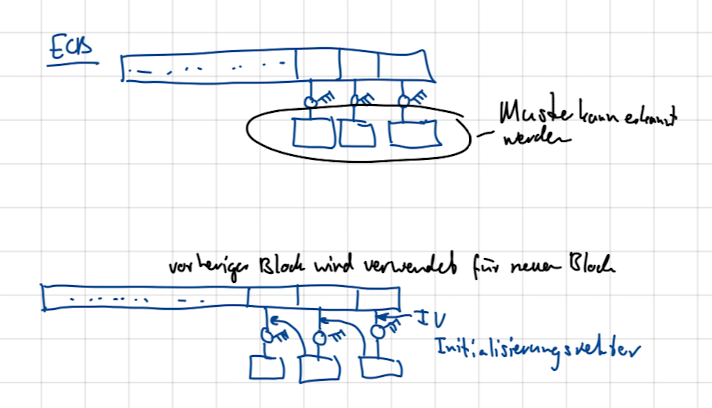
\includegraphics[width=12cm]{img/02_ecb.png}
\end{center}

\paragraph{Ciphern}
\begin{itemize}
\item \emph{AES} Schlüssellänge 256 verwenden (128 gebrochen); Blocklänge 128 andere existieren, werden aber seltener verwendet
\item \emph{Camelia} Feistelcipher mit Schlüssellänge 192, 256 (128 potenziell gebrochen); Blocklänge 128 Bit
\item \emph{Cast-256} ungebrochen; Schlüssellänge 256 (128, 169 192, 224 potenziell gebrochen); Blockgrösse 128 Bit
\end{itemize}

\paragraph{Hashing}
Einwegfunktion um Daten zu einer nicht rückverfolgbaren Zeichenfolge zu formen. Wird mit oder ohne Salt verwendet (Salt wird vor das Dokument gesetzt, welche unabhängig von den Daten ist). Ein Hash sagt nichts über die Eigenschaft eines Dokumentes aus, ist aber einzigartig.

Eine Rainbow-Table enthält alle möglichen Kombinationen von Hashes.

\paragraph{Hashing Verfahren}
\begin{itemize}
\item \emph{MD5} -- gebrochen
\item \emph{RIPE-MD 160} -- gebrochen
\item \emph{SHA1} -- gebrochen
\item \emph{SHA2/3 224} -- vermutlich gebrochen
\item \emph{RIPE-MD 256+}
\item \emph{SHA2/3 256+}
\end{itemize}

\subsection{Zertifikate}
Komponenten von Zertifikaten:
\begin{itemize}
\item \emph{Identifikation} -- Felder \emph{SubjectDN} und \emph{SubjectAlternateName}
\item \emph{Öffentliche Schlüssel} -- öffentlicher Teil eines asymmetrischen Schlüsselpaares; kann zum Prüfen von verschlüsseltem Material oder zum Verschlüsseln von Material an den Zerifikatsanbieter dienen
\item \emph{Gültigkeitsdauer} -- Startzeitpunkt und Endzeitpunkt
\item \emph{Verwendungszweck} -- Benutzung kann eingegrenzt werden; e.g. nur für Signatur von Emails oder Authentisierung von Web-Clients
\end{itemize}

\paragraph{Key- und Truststore}
Jede Applikation, die mit Zertifikaten arbeitet hat idR 2 Stores und folgenden Inhalt:
\begin{itemize}
\item \emph{Keystore} -- Zertifikate und den privaten Schlüssel
\item \emph{Truststore} -- Trust-Anker (Root-Zertifikate)
\end{itemize}



\newpage
\section{Verschlüsselung (Teil 2: PKI und andere Vertrauensmodelle}

\paragraph{Hybride Verschlüsselung und PFS} \emph{Perfect Forward Secrecy} gewährleistet, dass beim Bruch eines Langzeitschlüssels, die Kommunikation nicht retrospektiv entschlüsselt werden kann.

\subsection{Signieren}
Vom Dokument wird ein Hash generiert, welcher mit dem privaten Schlüssel verschlüsselt wird. Das Dokument wird unverschlüsselt zusammen mit dem verschlüsselten Hash an den Empfänger geschickt. Der Empfänger kann mit dem öffentlichen Schlüssel des Versenders den Hash prüfen.

\paragraph{Signieren mit OpenSSL}

\begin{center}
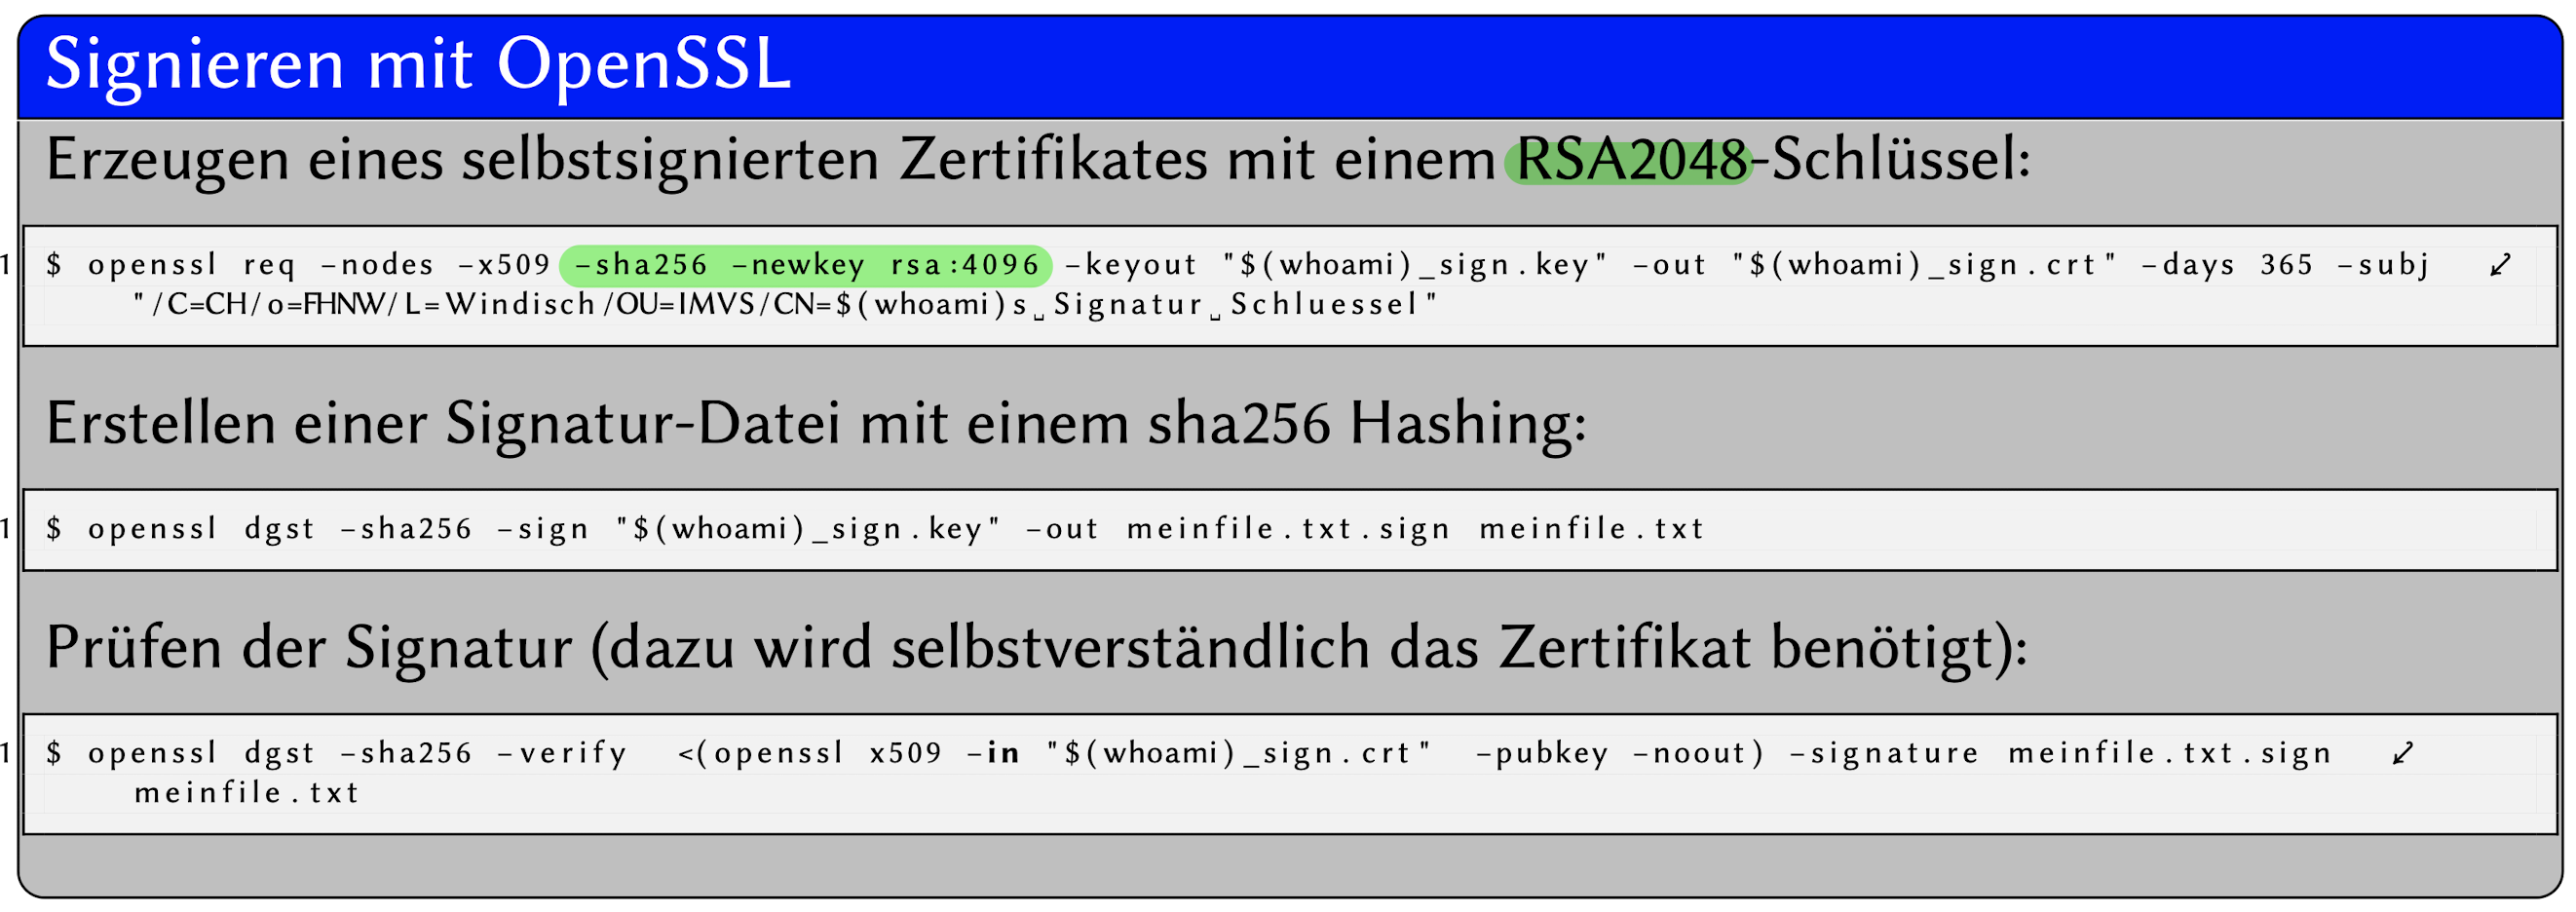
\includegraphics[width=12cm]{img/04_openssl.png}
\end{center}

\paragraph{Signieren mit PGP}

\begin{center}
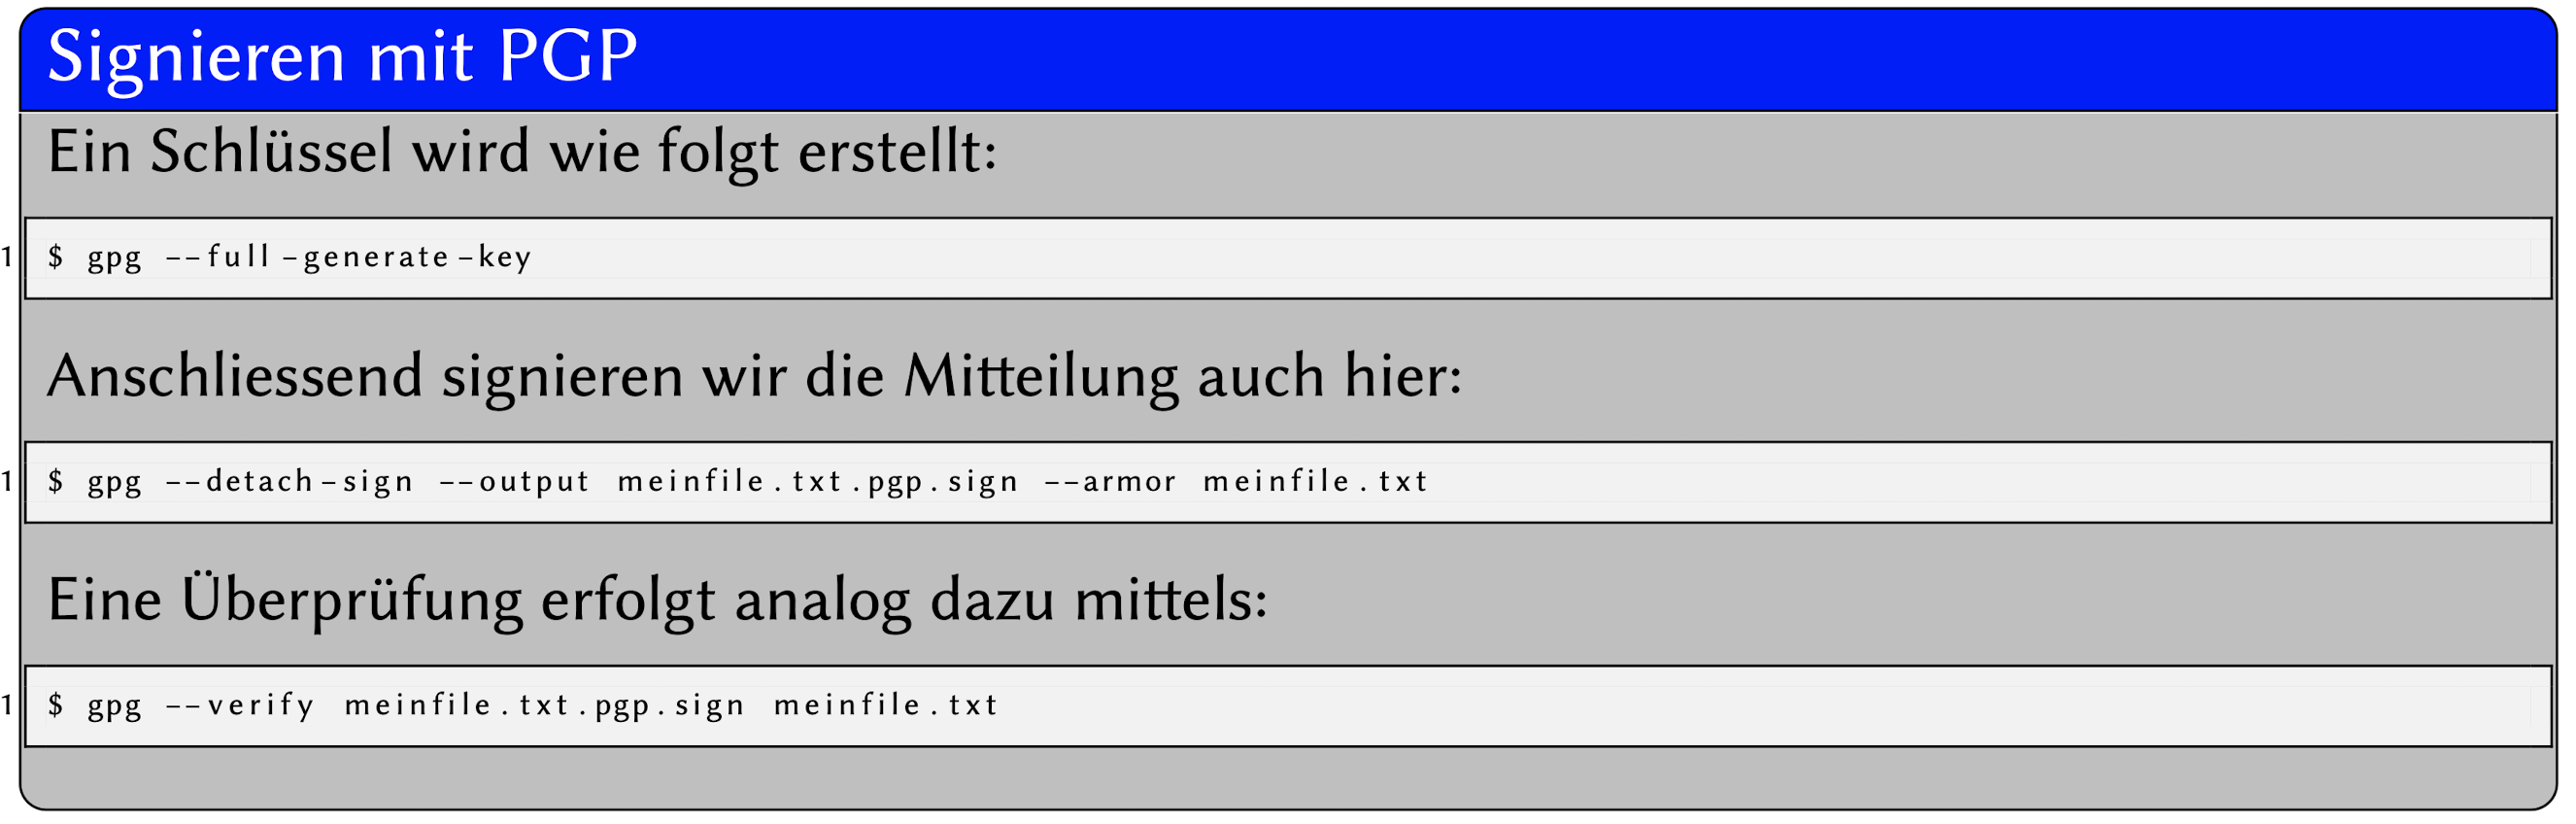
\includegraphics[width=12cm]{img/04_pgp.png}
\end{center}

\paragraph{Signieren einer Mitteilung}

\begin{center}
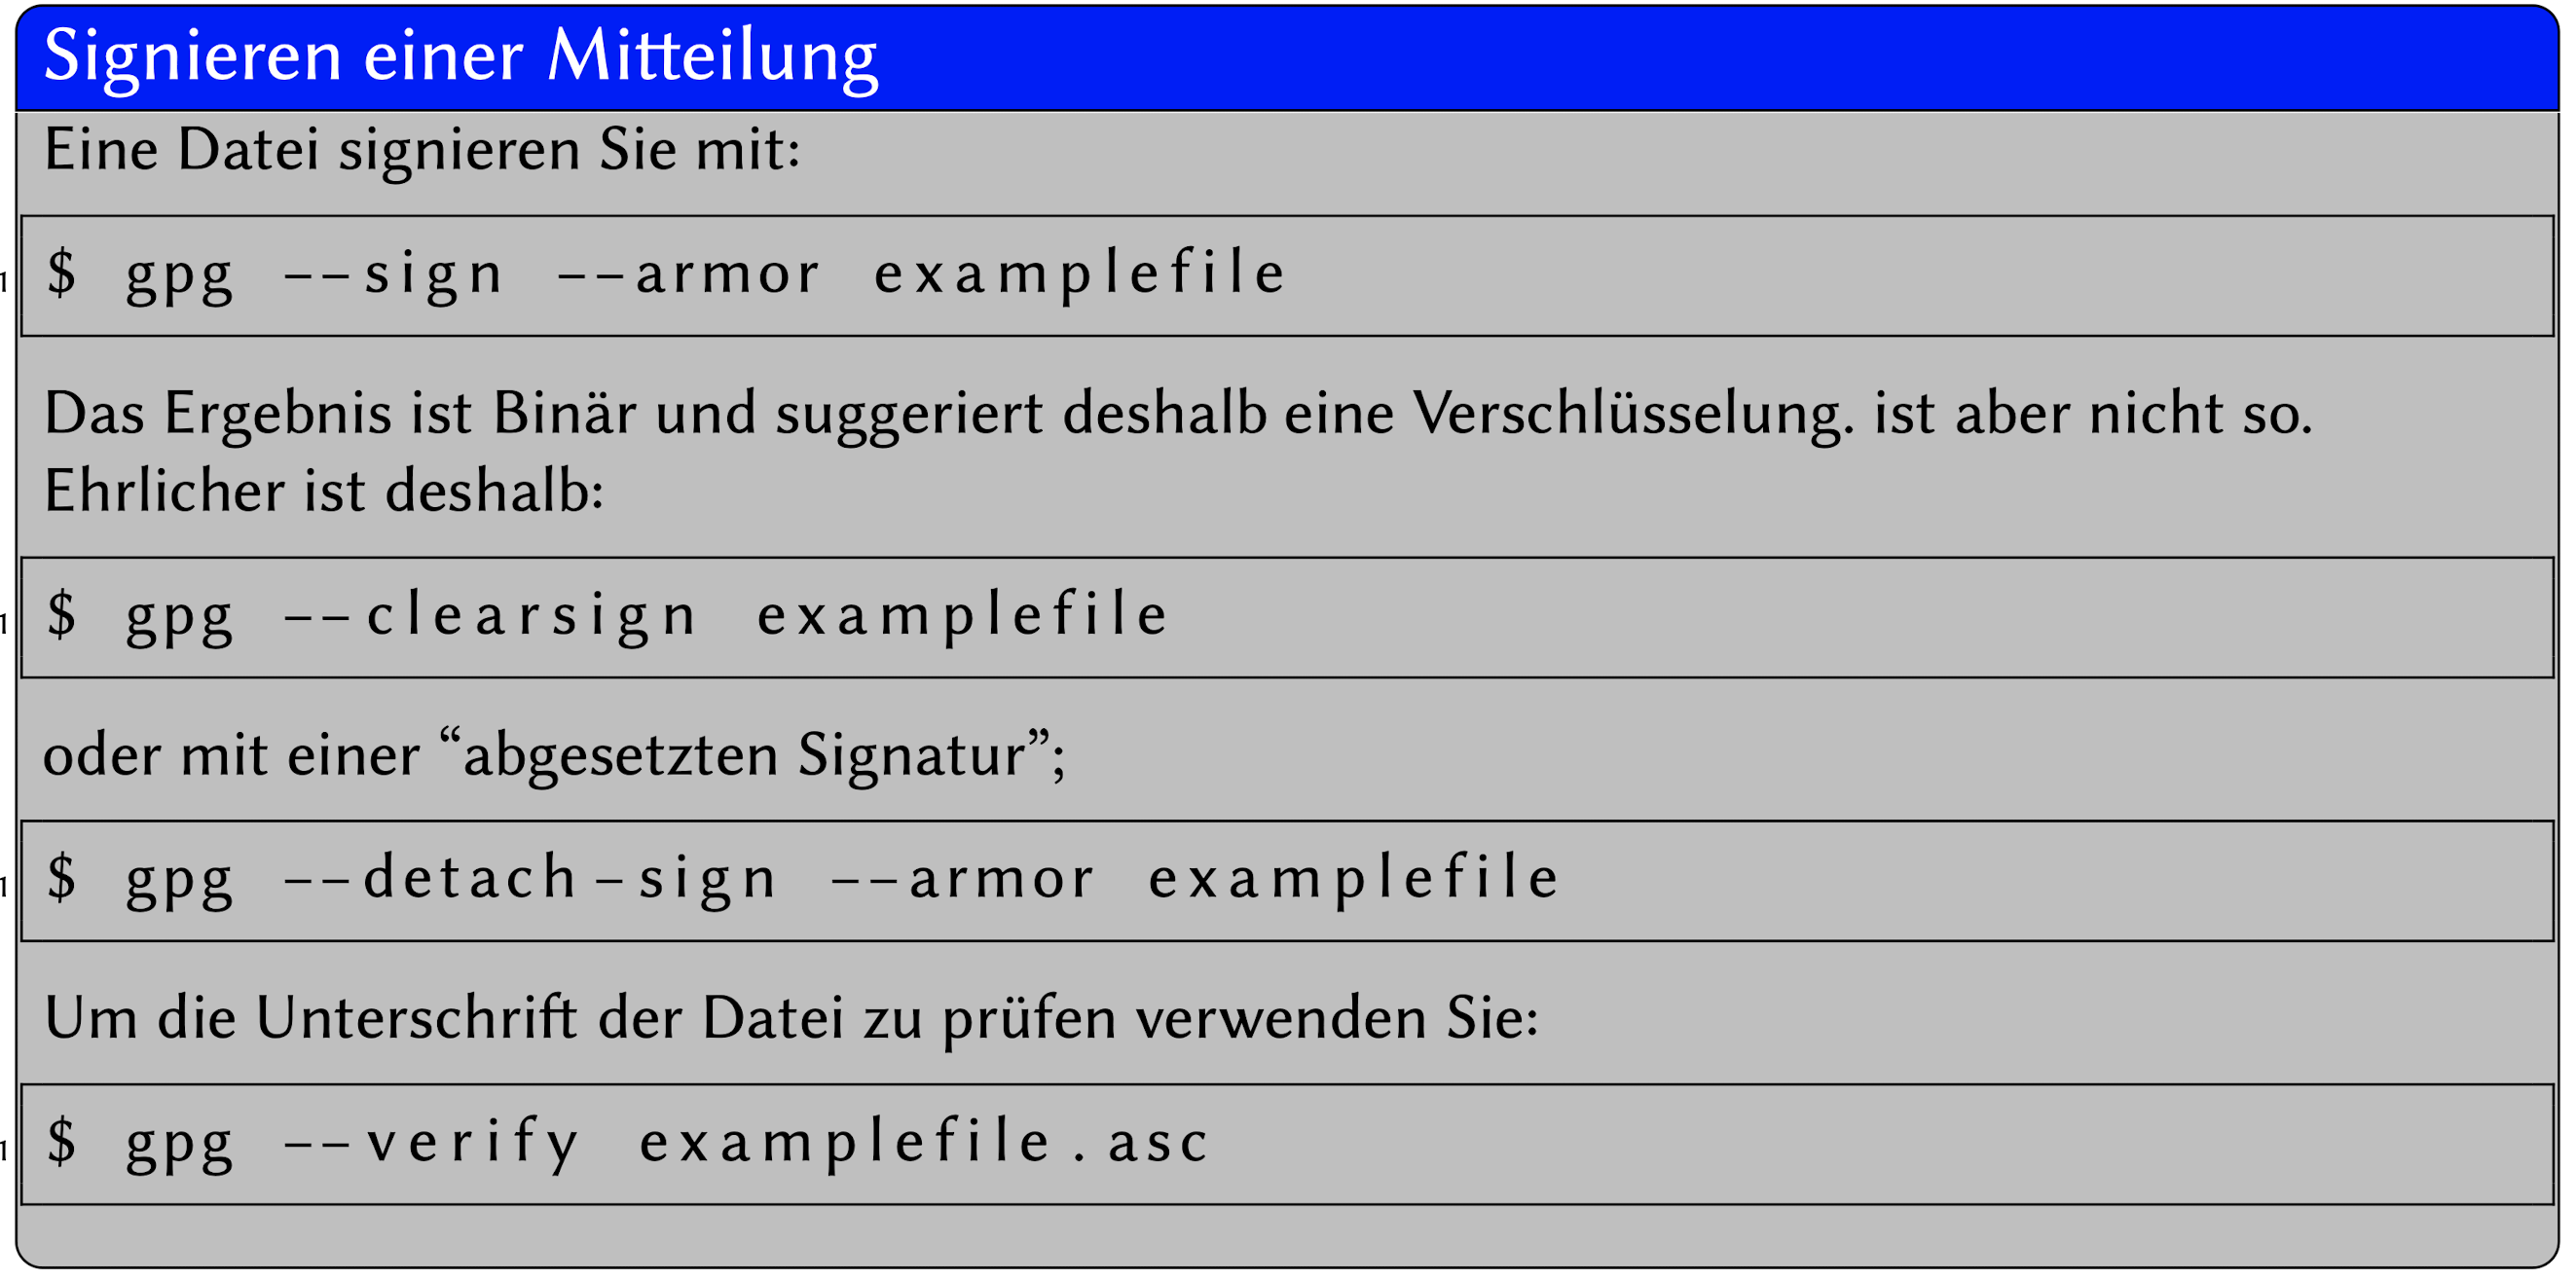
\includegraphics[width=12cm]{img/04_pgp_1.png}
\end{center}

\paragraph{Passworte "sicher" via Netzwerk prüfen}

\begin{center}
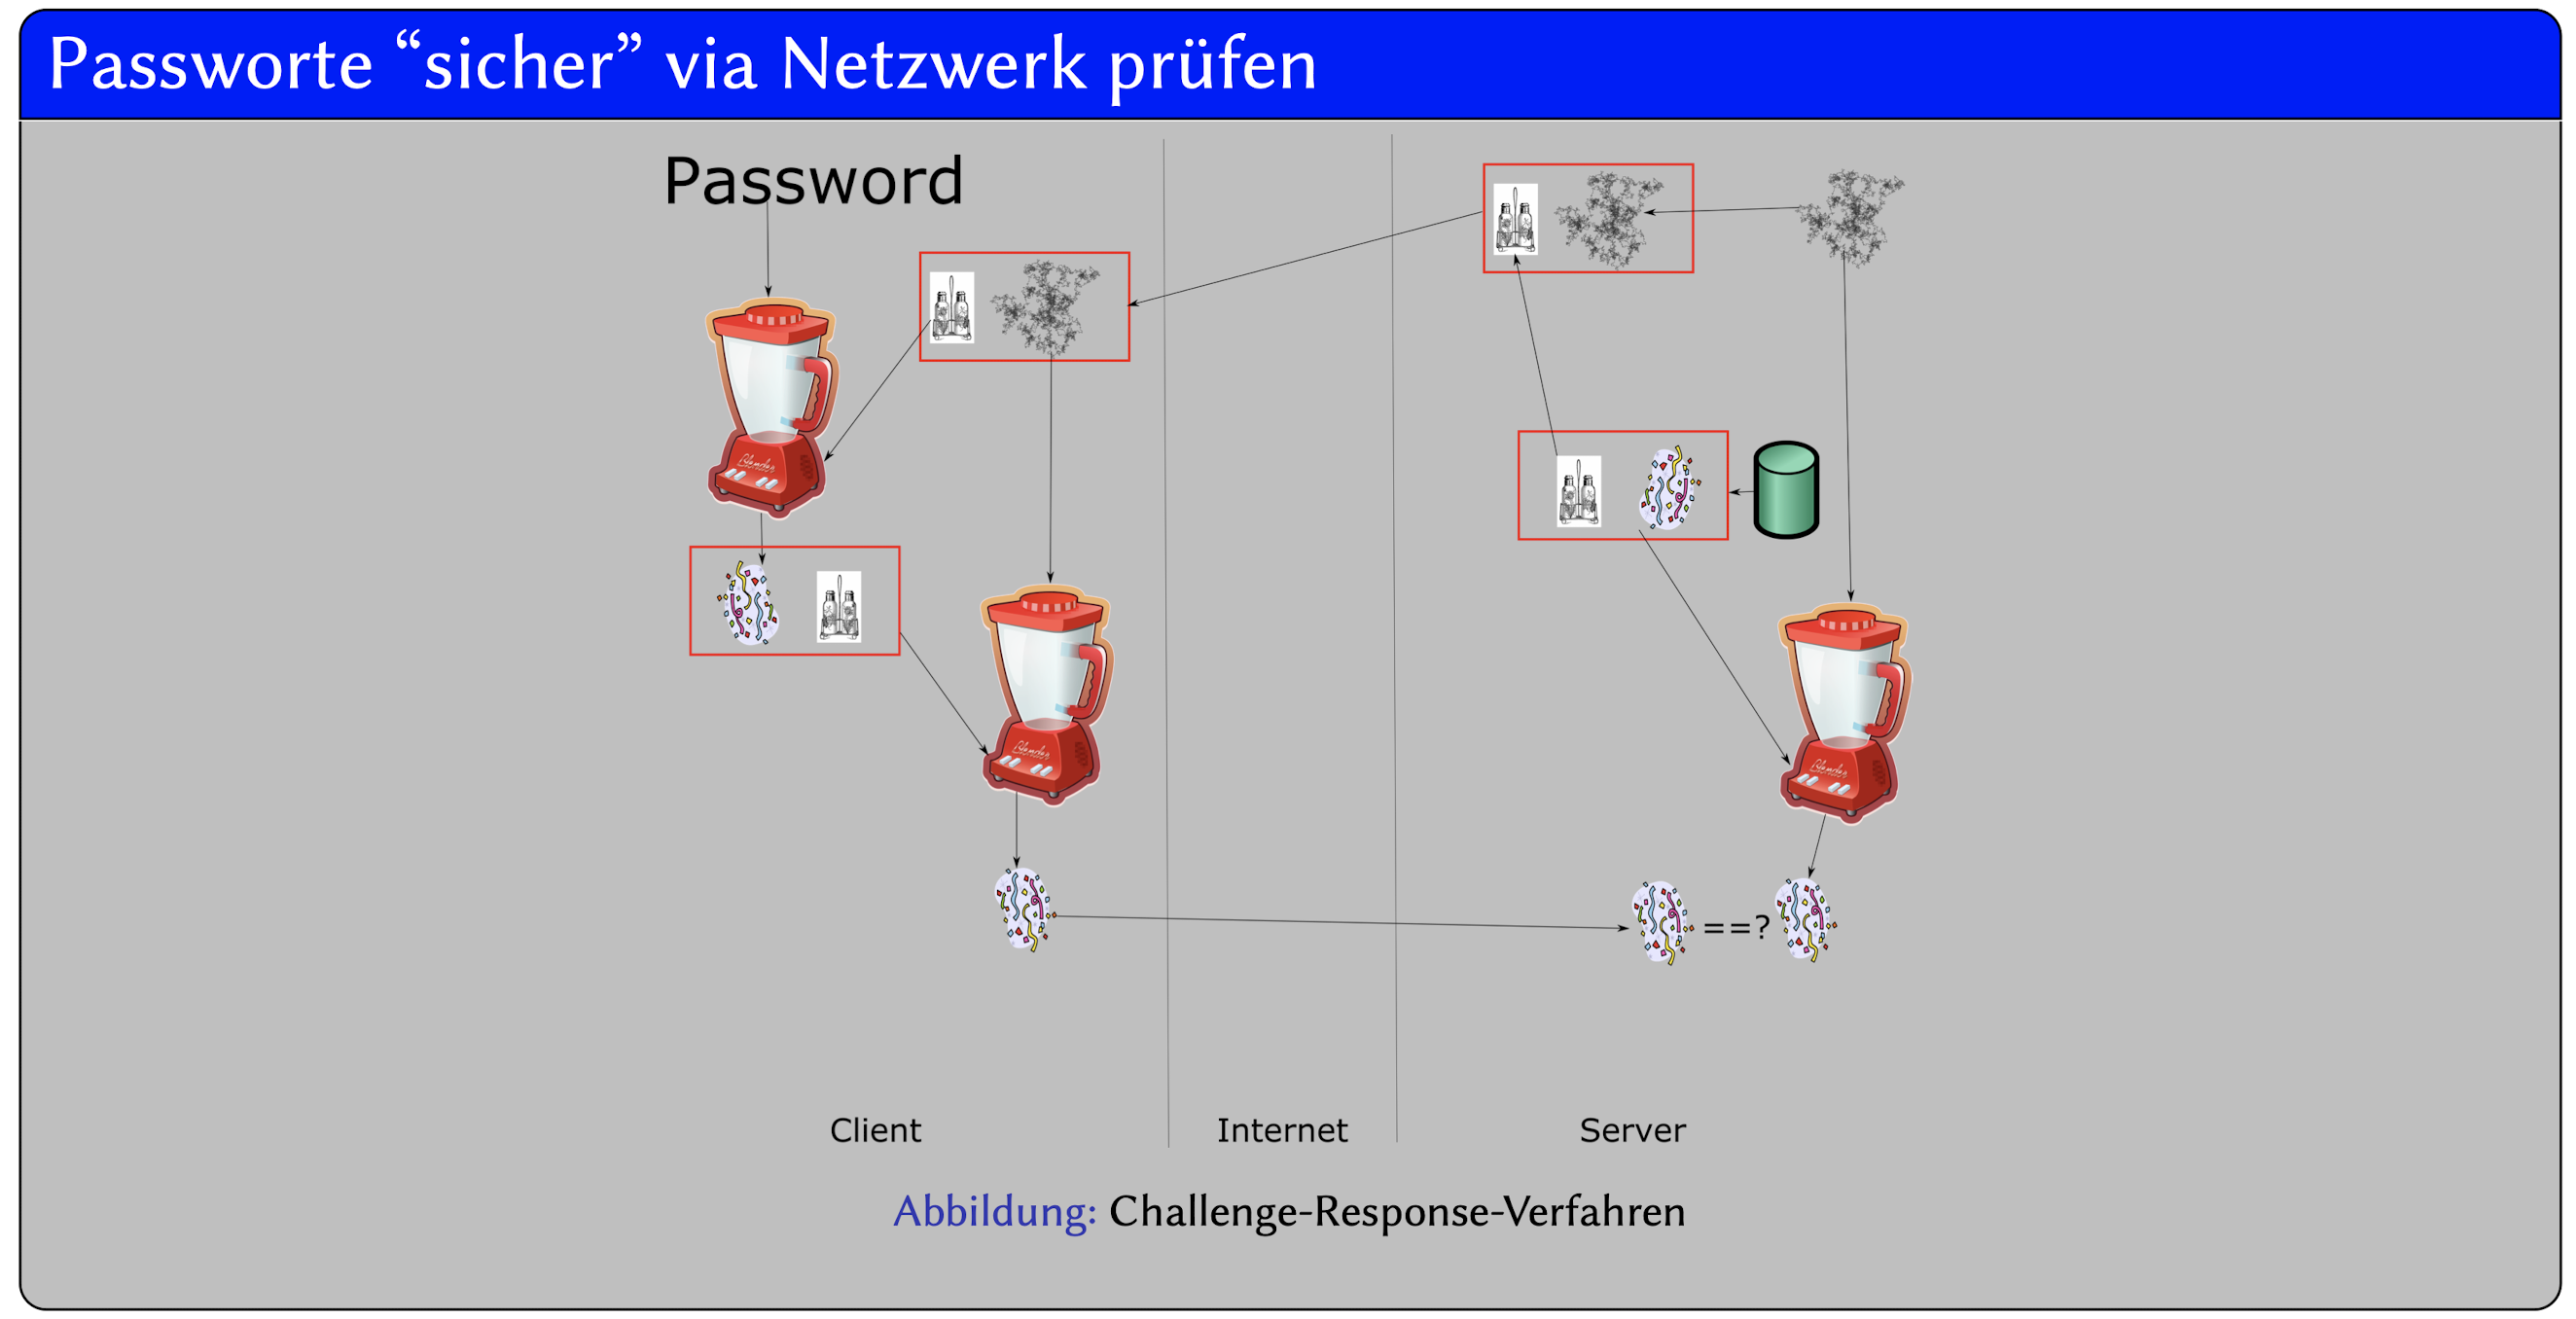
\includegraphics[width=12cm]{img/04_transfer.png}
\end{center}


\paragraph{Zero Knowledge Proof (ZKP)} Prüfer (P / Peggy) beweisen den Besitz eines Passwortes, ohne dass die verifizierende Instanz durch den Prüfvorgang zusätzliche Kenntnisse über das Passwort erhält. Drei Phasen:
\begin{itemize}
\item Peggy legt ein Commitment vor -- mehrere richtige Antworten über ein Zusammenhang
\item Victor fordert die Aufdeckung einer Antwort aus dem Commitment -- Resultatsets überlappen sich
\item Peggy deckt die Antwort auf
\end{itemize}




\newpage
\section{Zertifikate}

\paragraph{Begriffe}
\begin{itemize}
\item \emph{Zertifikat} -- Überprüfbarer Schlüssel der einem Verwendungszweck dient; Meistens ein unterschriebener Public Key
\item \emph{Certification Authority (CA)} -- Instanz, die Zertifikate ausstelt
\item \emph{Registration Authority (RA)} -- Instanz, bei der Zertifikate beantragt werden können und die den Antrag prüft
\item \emph{Certification Revocation List (CRL)} -- Liste von Zertifikaten, die nicht mehr gültig sind
\item \emph{Validation Authority (VA)} -- Instanz, die Zertifikate prüft; Überprüfung ist ein vollautomatischer Prozess
\end{itemize}

\subsection{Public Key Infrastructure (PKI)}
Eine PKI ist ein System, dass digitale Zertifikate ausstellen, verteilen und prüfen kann.

Vertrauensmodelle:
\begin{itemize}
\item \emph{Hierarschisch} -- Vertrauensstellung in eine CA. Jedes von ihr unterschriebene Zertifikat ist für die im Zertifikat angegebenen Aktionen gültig. Die CA unterschreibt ihr eigenes Zertifikat.
\item \emph{Web of Trust} -- Zertifikate drücken sich gegenseitig ihr Vertrauen aus; jedem selber überlassen, wie Vertrauen definiert ist (e.g. PGP)
\item \emph{Cross Zertifizierung} -- Zwei CA unterschreiben ihr Zertifikat; Vertrauensstellung nicht immer eindeutig geregelt und kann von Fall zu Fall variieren
\end{itemize}

\paragraph{Dokumente}
\begin{itemize}
\item \emph{Certificate Policy (CP)} -- Beschreibt die Anforderungen an die CA und ihre Arbeitsweise; dient dritten zur Analyse der Vertrauenswürdigkeit
\item \emph{Certificate Practice Statement (CPS)} -- Beschreibt die praktische Umsetzung des CP Dokumentes un die Praxis; unter welchen Bedingungen ein Zertifikat ausgestellt wird; Wenn CPS nicht öffentlich ist, gibt es noch ein Policy / PKI Disclosure Statement (PDS), welches den öffentlichen Teil enthält
\end{itemize}

\paragraph{PKI}

\begin{center}
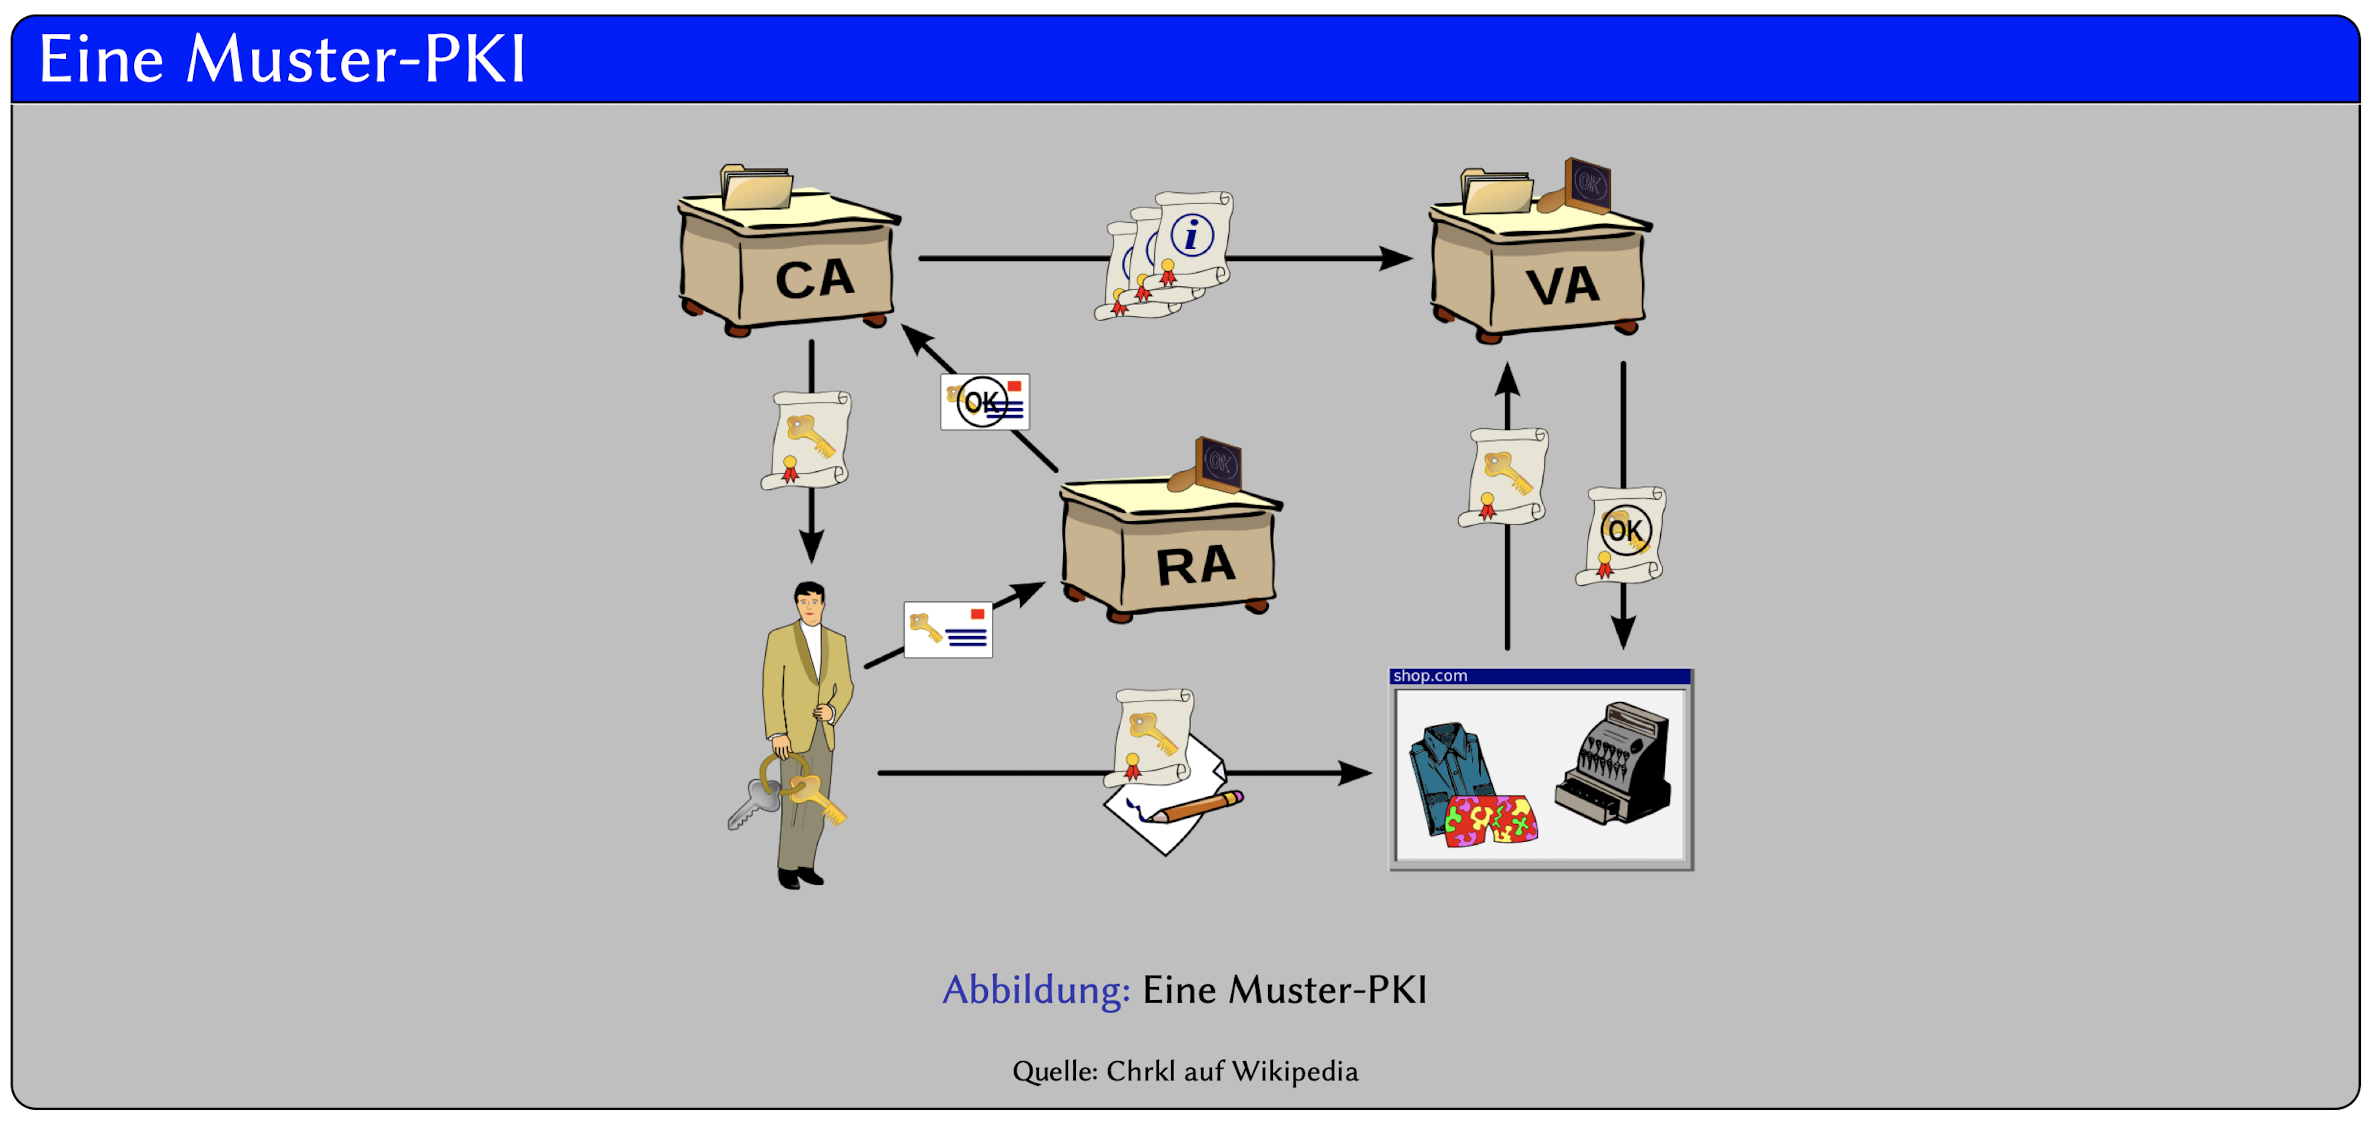
\includegraphics[width=12cm]{img/05_pki.png}
\end{center}

\subsection{Verschlüsselte Verbindungen}

Aufbau von Verbindungen kann verschiedene Fehler darstellen:
\begin{itemize}
\item Nicht vertrauenswürdige Root-Zertifikate 
\item Abgelaufene oder zurückgezogene Zertifikate
\item Verwendung eines Zertifikates, das nicht dafür zugelassen ist
\end{itemize}

\paragraph{Vertrauensverhältnis mit OpenSSL analysieren}

\begin{center}
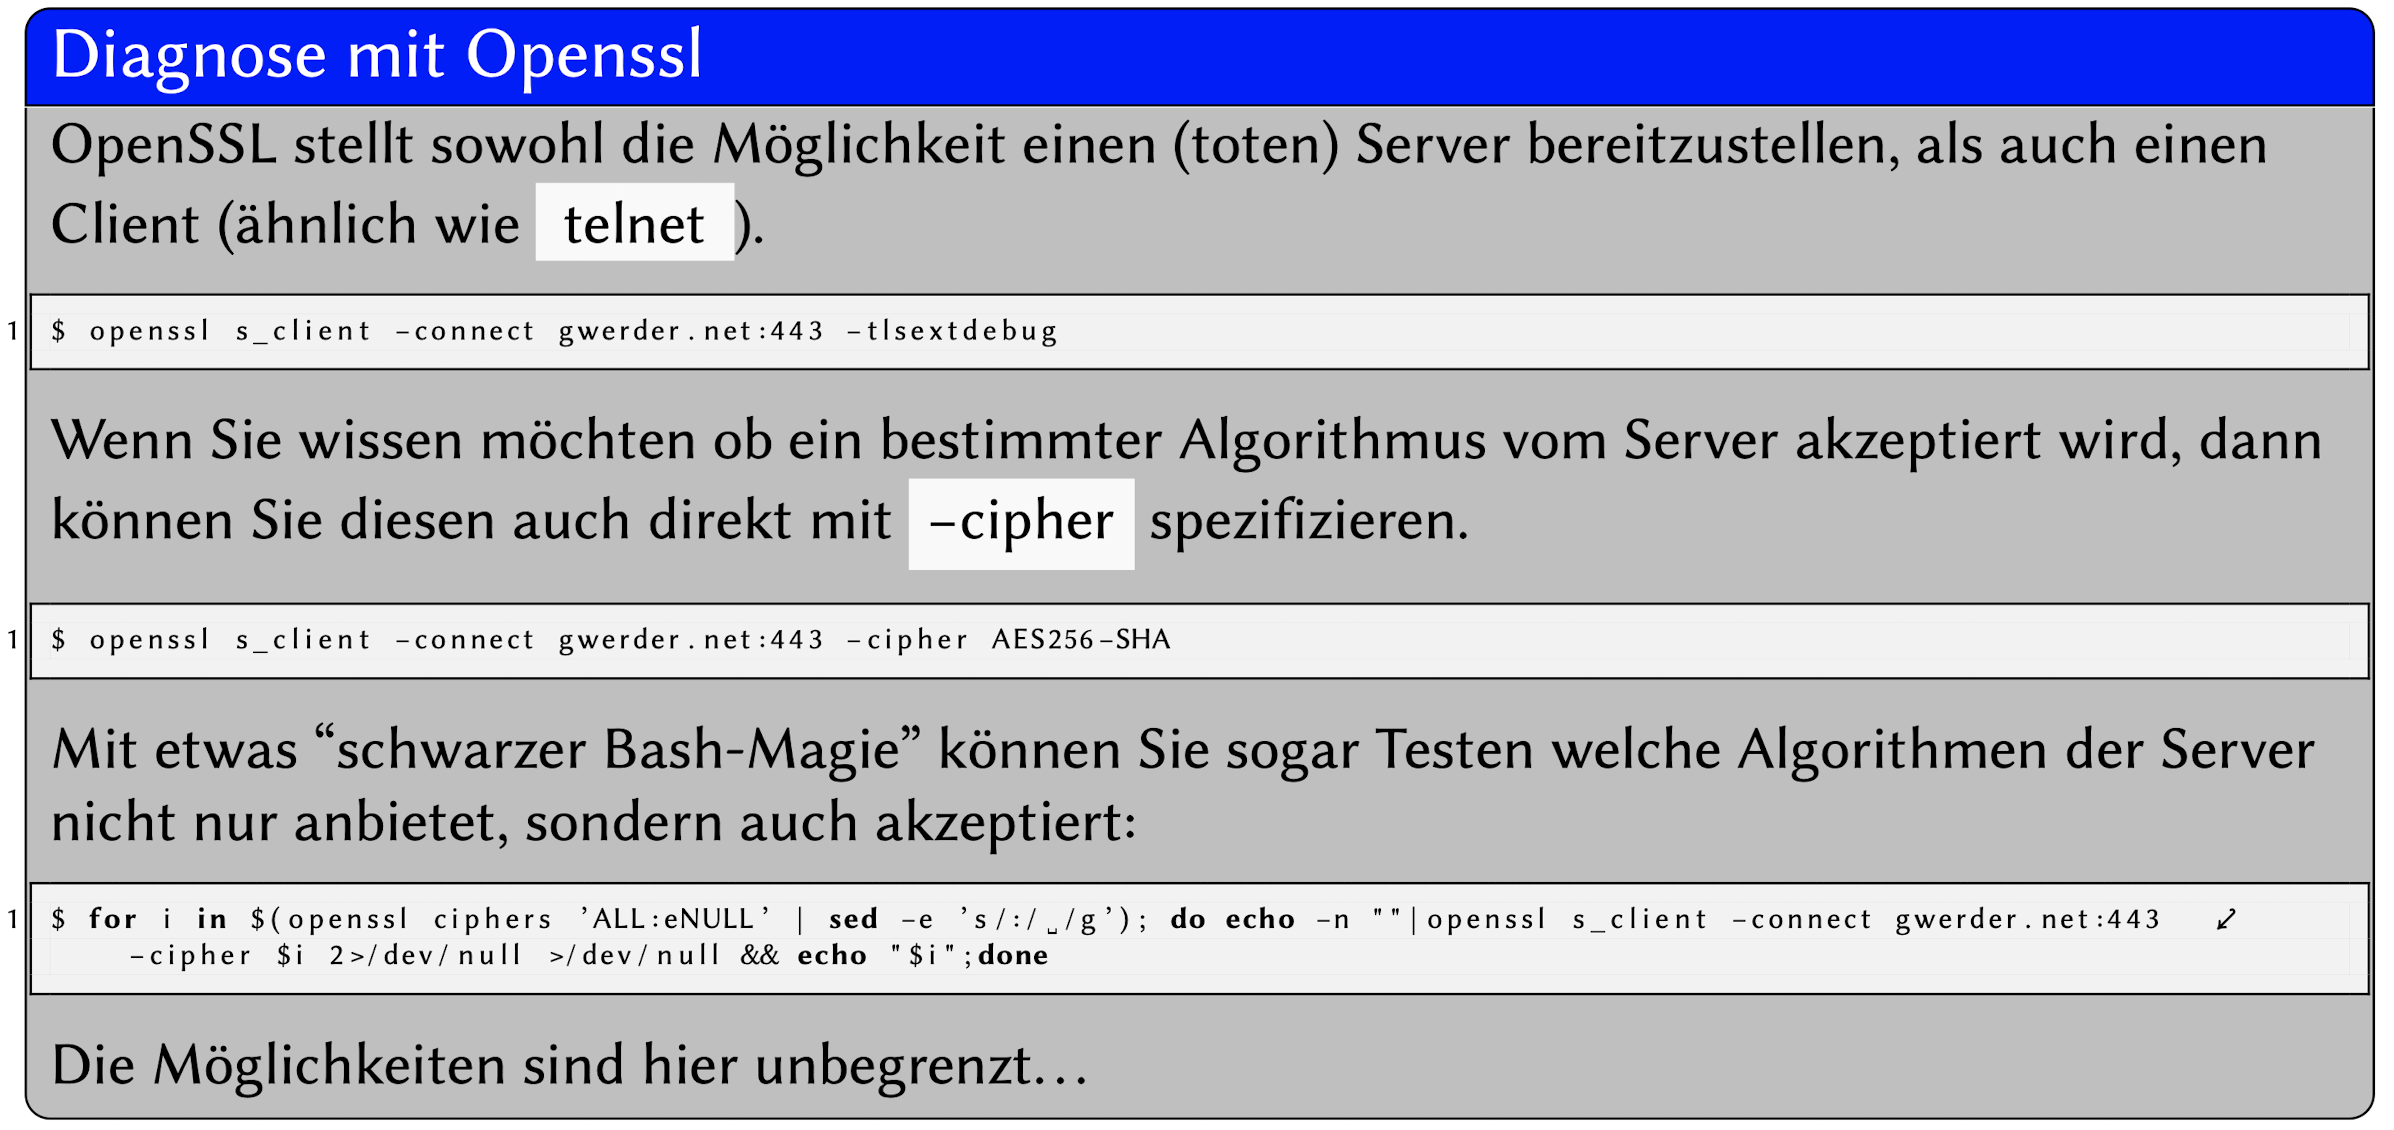
\includegraphics[width=12cm]{img/05_openssl.png}
\end{center}

Es können auch Server-Verbindungen erstellt werden, um einen Client zu diagnostizieren -- \emph{Ein Server benötigt immer ein Zertifikat}

\begin{center}
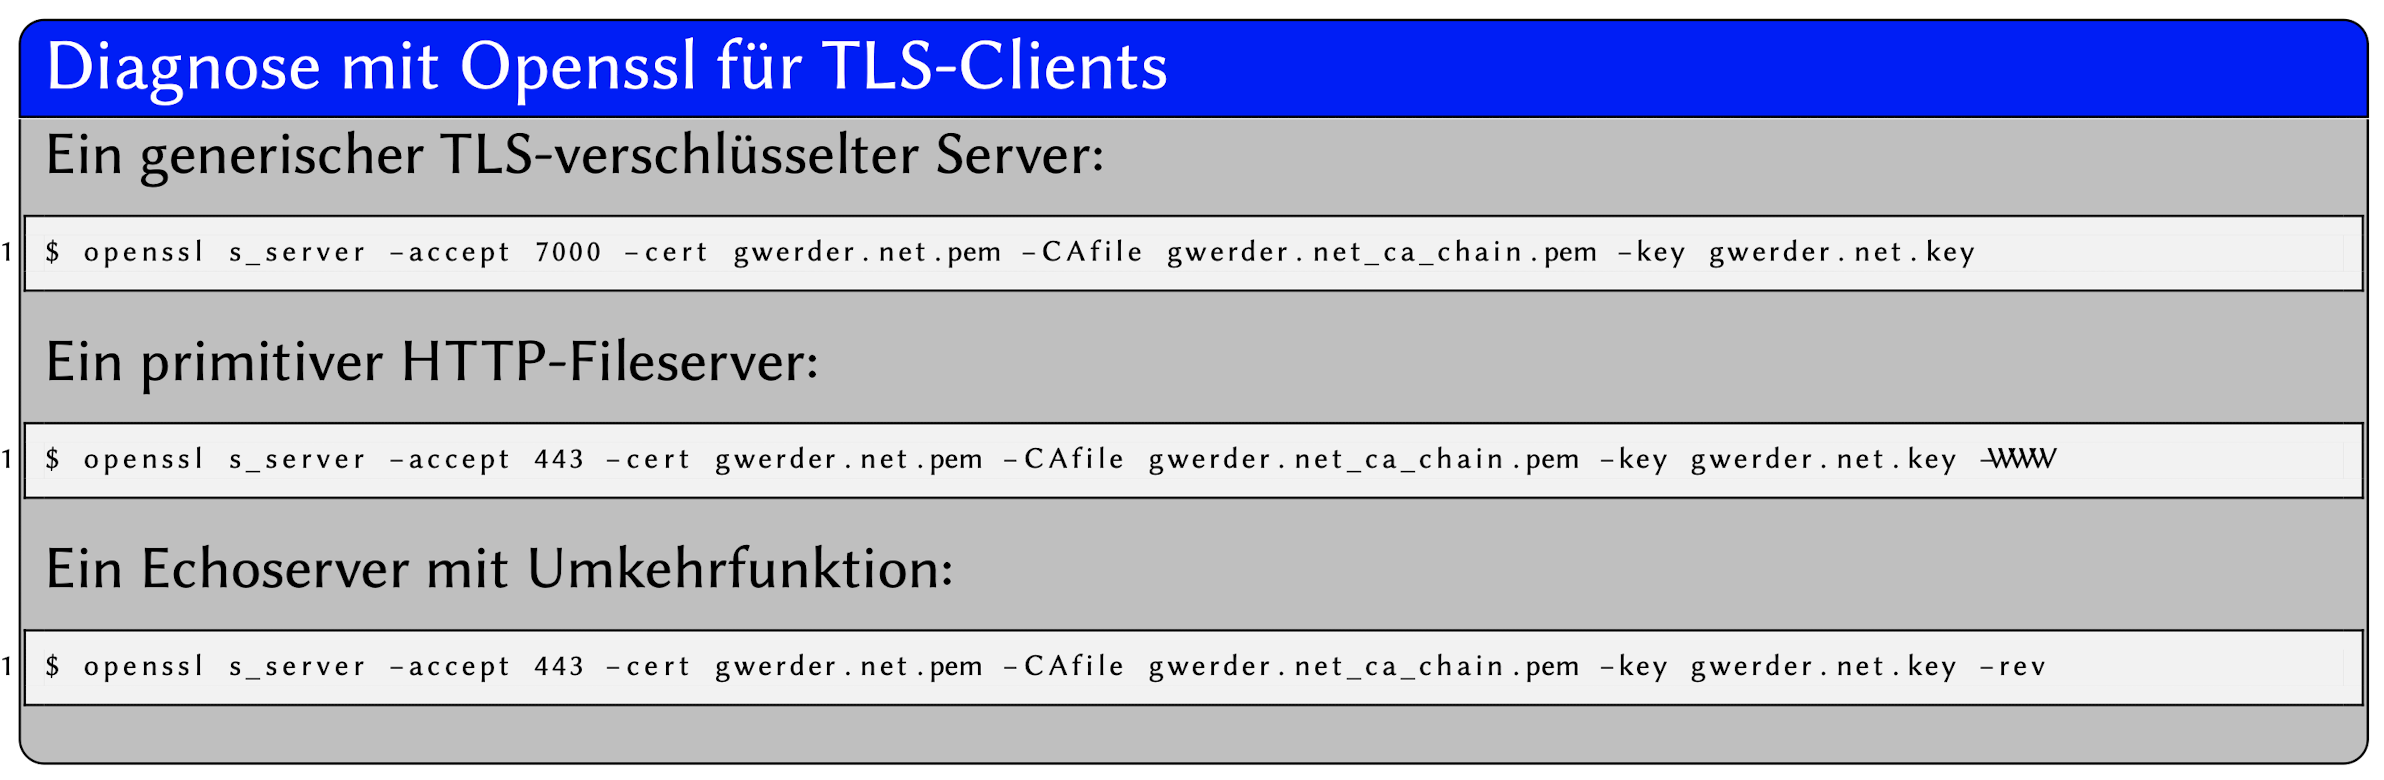
\includegraphics[width=12cm]{img/05_openssl_2.png}
\end{center}
\begin{center}
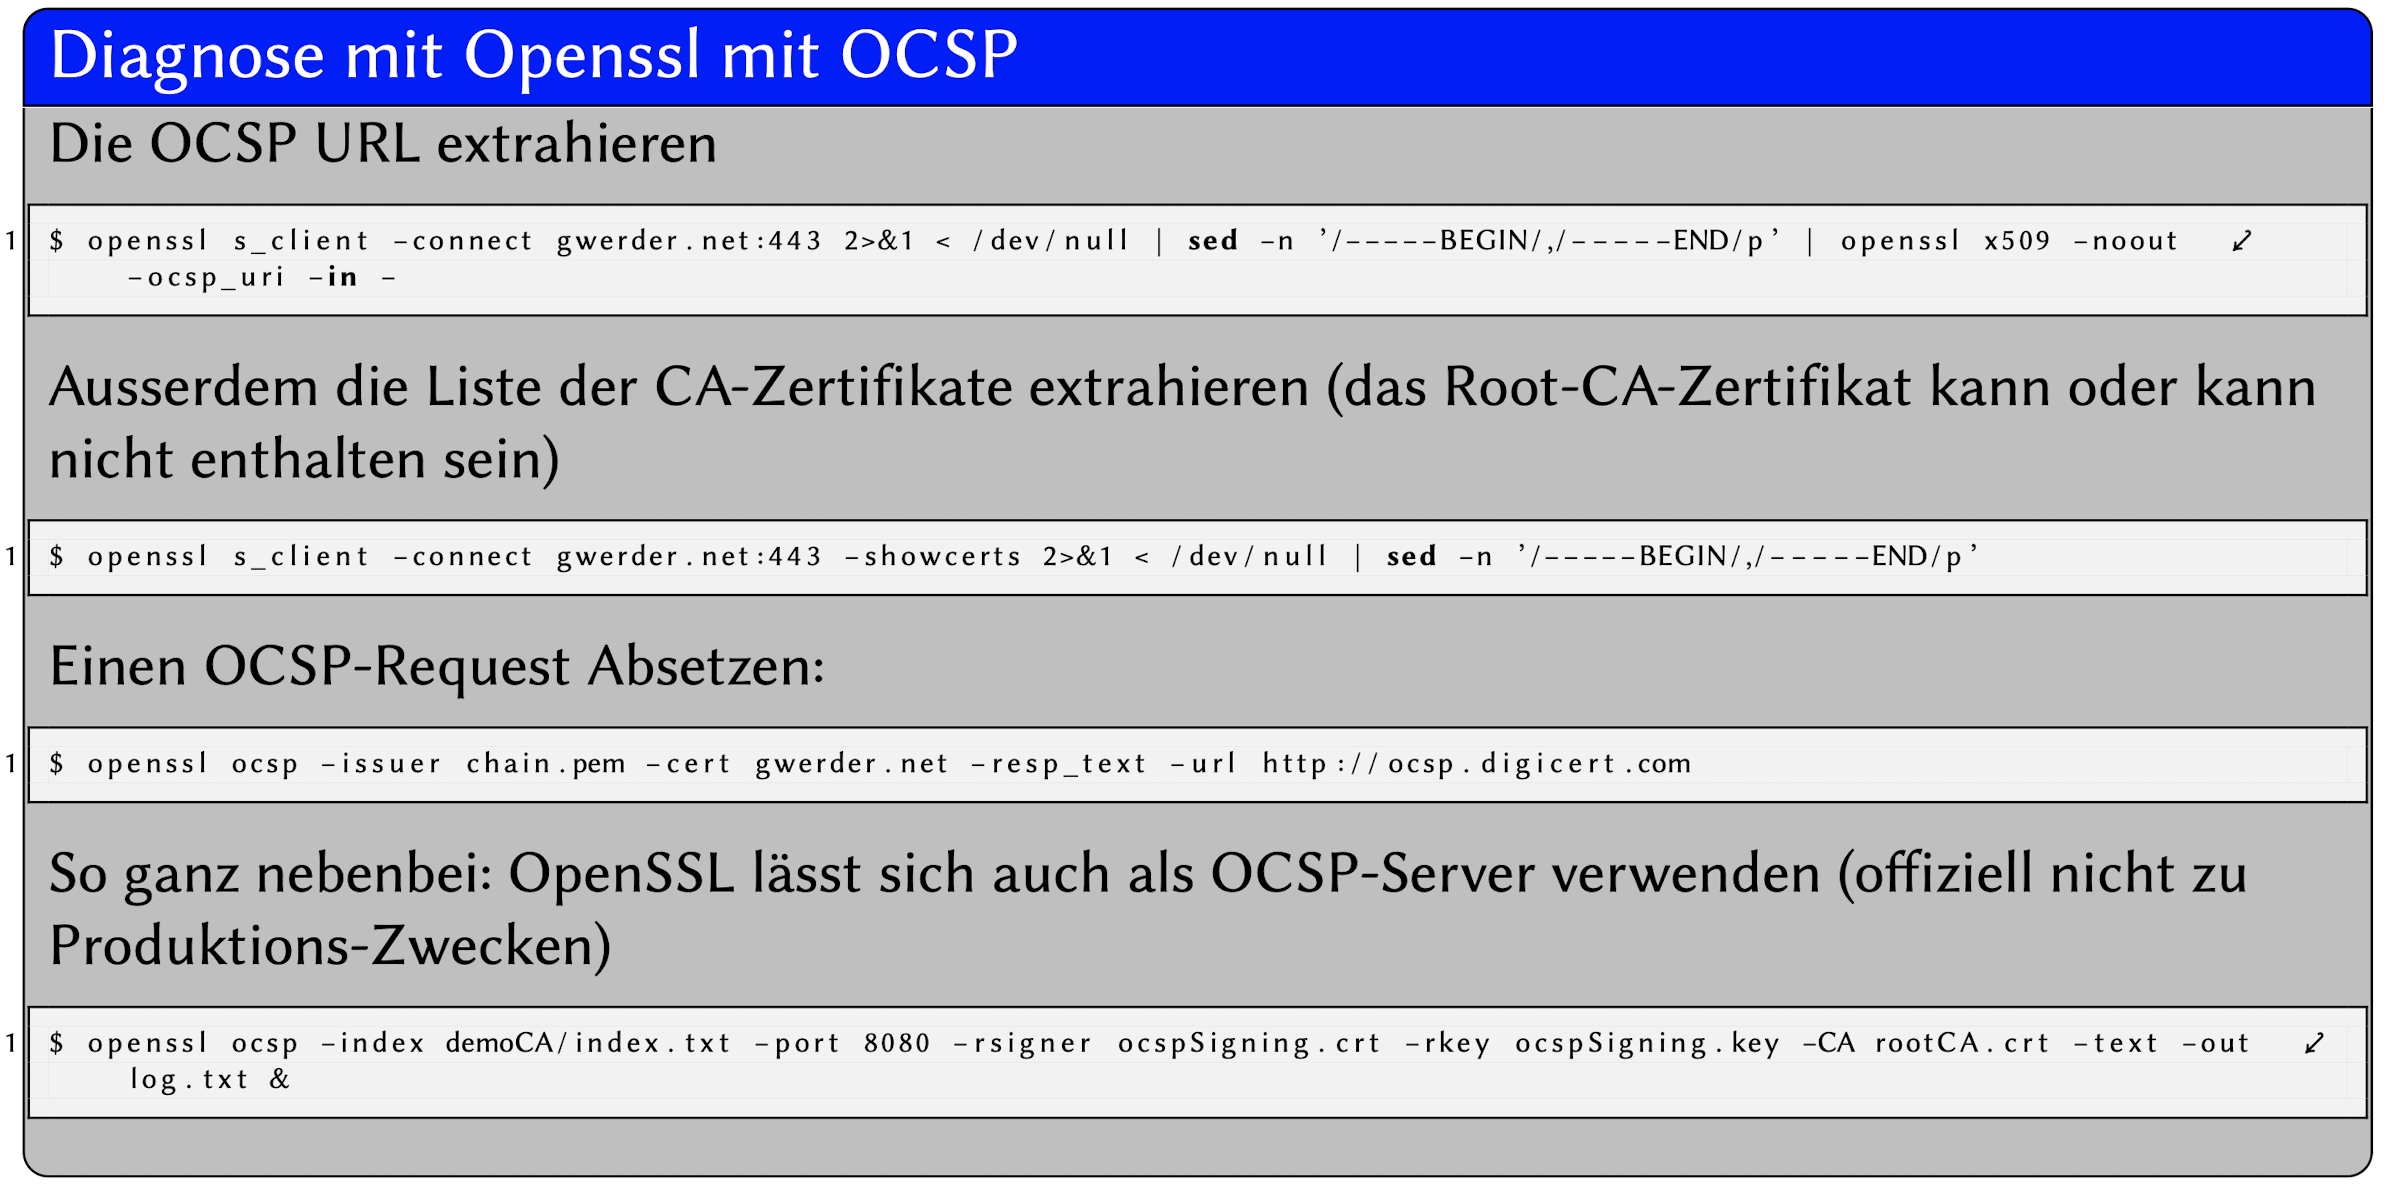
\includegraphics[width=12cm]{img/05_openssl_3.png}
\end{center}

\subsection{Security Tokens}
Security Tokens sind ein wichtiger Faktor bei Mehrfaktor-Authentifizierung

\begin{itemize}
\item \emph{Zeitsynchronisierte Tokens} -- Präsentieren einen OTP aus ggw. Zeit und einem Geheimnis
\item \emph{CR-Basierte Tokens} -- Eingabe einer Challenge erfolgt über eine Schnittstelle; Challenge wird mit dem Schlüssel der Person "signiert" und zutückgesandt
\item \emph{Usage Based Tokens} -- Eine Art "Streichliste"; Bei jedem Druck auf eine Taste wird der nächste Code freigegeben; vorhergehende Codes werden automatisch invalidiert
\end{itemize}

\paragraph{Verbinden von Security Tokens}
Security Tokens sind in verschiedenen Varianten verfügbar
\begin{itemize}
\item Online -- via USB; NFC; Fest auf einem Gerät verbaut
\item Offline -- Eingabe über Tastatur oder via Telefon
\end{itemize}

Wenn ein Token online ist, ist bei sicheren Tokens eine manuelle Aktion nötig um den Authentisierungsvorgang zu imitieren

\paragraph{Kritik}

\begin{itemize}
\item \emph{Verluste oder Diebstahl} -- Verlust oder Diebstahl grundsätzlich kein Problem; muss mit den entsprechenden Massnahmen begleitet werden
\item \emph{Man-in-the-Middle} -- Die meisten Smarttokens überprüfen nicht ihren Peer-Partner; Authentisierungs-Tokens sind anfällig für MITM wenn nicht anderweitig abgesichert
\end{itemize}








\newpage
\section{Technische und nicht-technische Angriffe}
Es gibt mehrere Möglichkeiten Ereignisse zu klassifizieren.


Abwehrstrategien:
\begin{itemize}
\item Angriff verhindern
\item Angriff erschweren
\item Angriff ableiten (intern oder extern)
\item Schaden kontrollieren
\item Angriff entdecken (während und danach)
\item Vom Angriff erholen
\end{itemize}



\subsection{Nicht-Technische Angriffe}
Angriffe, die ein Schutzziel beeinträchtigen können und als Ziel keine technische Anlage haben. Ziele sind Menschen, Prozesse, Zustände.

\paragraph{Dumpster Diving} vertrauliche Informationen werden über Abfall, Altpapier, ausrangierte Hardwareoder vergleichbare Kanäle besorgt; Sonderform über Webarchiv in der Vergangenheit publizierte Informationen beschaffen

\paragraph{Spying / Eavesdropping} Informationen werden beschafft, indem Beobachtungen angestellt werden, ohne dass Entitäten manipuliert werden. Beobachtungen können visuell, akustisch, technisch sein; \emph{Eavesdropping} ist, wenn Informationen über das Mitschneiden von legitimen Datenflüssen beschafft werden

\paragraph{Social Engineering} Menschen manipulieren um Sicherheitssperren zu umgehen. Mithilfe:
\begin{itemize}
\item Impersonation
\item Tailgating
\item Phishing / Vishing / Whaling
\item Popup Fenster
\item Interessante Applikationen
\item Hoaxing
\end{itemize}

\emph{Angriffskanäle} -- Email, Telefon, Soziale Medien, SMS, Brief, direkt
\emph{Gegenmassnahmen} -- Ausbildung aller Beteiligten; Etablieren von geeigneten Prozessen


\subsection{Technische Angriffe}
Klassifikation nach
\begin{itemize}
\item Schutzziel
\item Strategie
\item Schweregrad des potentiellen Schadens
\item Wahrscheinlichkeit
\item Komplexität
\end{itemize}

\paragraph{Gegenmassnahmen} 
\begin{itemize}
\item Zugriff aus die Systeme limitieren -- \emph{verhindern}
\item Angriffsfläche gering halten -- \emph{erschweren, kontrollieren}
\item Schadaktivitäten erkennen -- \emph{entdecken}
\item Potentiellen Schaden gering halten -- \emph{ableiten, erholen}
\end{itemize}

\paragraph{Phasen}
Angriffe werden selten isoliert sondern koordiniert geführt. Phasen von Attacken \emph{1)} Reconnaissance, \emph{2)} Exploitation, \emph{3)} Reinforcement, \emph{4)} Covering Tracks

\paragraph{(Distributed) Denial-of-Service} 
Bei der DoS-attacke geht es darum, ein Ziel vorübergehen oder bleibend vom Netzwerk zu schädigen. Die einfachsten Angriffe verursachen Überlastungen in einem Teilsystem. Fortgeschrittene Attacken zerstören Daten / Programme oder Hardware.

\paragraph{Man in the Middle} Dritter klinkt sich in Konversation ein; lässt sich durch \emph{Mutual Authentication} verhindern. Bei Man in the Browser kontrolliert der Angreifer einen der Endpunkte (nach der abgesicherten Verbindung. 



\newpage
\section{Angriffe und Szenarien}
Verschiedene Arten von Exploits: technische Möglichkeit, Schachstellen eines Programms oder Hardware auszunutzen. Viele Arten von Exploits: \emph{1)} Remote Code Execution, \emph{2)} Local Privilege Escalation, \emph{3)} Information Disclosure / Manipulation.

Alle Exploits können Attribute aufweisen. Für Angreifer sind Exploits am attraktivsten, die öffentlich nicht bekannt sind.


\paragraph{Responsible Disclosure} Schwachstellen werden oft einer \emph{Responsible Disclosure} unterworfen. Anfänglich wird nur publiziert, dass eine Schwäche in einem System oder Software hat und wie gravierend sie ist. Details werden dem Herstelle oder Verantwortlichen zugänglich gemacht.

Gegenseitig dazu ist \emph{Full Disclosure}, wenn Informationen schnellstmöglich breit zugänglich gemacht werden. Somit haben Täter und Opfer den selben Wissensstand.

\paragraph{Zero Day Exploit}
Schwachstellen, die durch die Entdeckung durch eine Malware von der Öffentlichkeit entdeckt werden.


\subsection{Angriff}
\begin{itemize}
\item \emph{(Cache-)Poisoning} -- mittels falscher Informationen Datenströme umleiten: DNS-Poisoning, ARP-Spoofing, DHCP-Poisoning
\item \emph{Erpressung} -- Typischerweise \emph{Ransomware}; Existiert auch über den Verkauf von gebrauchten Festplatten
\item \emph{Privilege Escalation} -- Sicherheitsbarrieren umgehen; Übernahme von Rechten hochprivilegierter Prozesse oder durch Überwindung von Sicherheitsbarrieren
\end{itemize}

\paragraph{Webbasierte Angriffe}
Häufigste Angriffe sind: \emph{1)} Drive-by-Infektionen, \emph{2)} Injection Attacken (Cross-Site-Scripting, SQL-Injektion)

\begin{itemize}
\item \emph{Persistent} -- In einem Blog, Kommentarfunktion, Gästebuch; e.g. über Upload von Files, Verlinkung von ungeprüften Quellen
\item \emph{Non-Persistent} -- Einfachste Attacke; untergeschobener Link meistens im Zusammenhang mit einem Phising-Mail
\item \emph{DOM-Based} -- Untergeschobener Link wird aus dem DOM des Browsers geladen
\end{itemize}


\paragraph{Directory / Path-Traversal-Attack} Lokale Files werden ausserhalb des Server-Roots geladen und übermittelt über \emph{1)} Backreferencing, \emph{2)} Logische Links.


\paragraph{CVSS Scores} Geben den Schweregrad einer gefundenen Schwachstelle an
\begin{itemize}
\item \emph{Basis Metrik} -- Grundsätzliches über Exploit
\item \emph{Zeitbasierte Metrik} -- Ändern sich über die Zeit
\item \emph{Umfeld-Metrik} -- Firmenspezifisch / Setup-Spezifisch
\end{itemize}



\newpage
\section{Malware}

\subsection{Angriffe Entdecken}

\paragraph{Indikatoren} Zwei Arten: \emph{1)} Indikatoren für einen Angriff (IOA) und \emph{2)} Indikatoren für eine Kompromittierung.
Ist grundsätzlich nicht das Selbe.

Häufigste Gefahr: Verschlüsselnde Ransomware -- verschlüsselt alles bevor sie entdeckt werden kann. Höchste Gefährdung. 

Die Indikatoren sind abhängig vom eigenen System. 

\paragraph{Indikatoren für einen Angriff (IOA)}
Bei Angriff: \emph{Sammeln} und dann \emph{Analysieren}.

\begin{itemize}
\item Versagen eines Dienstes oder Zerstörung eines Assets
\item Geänderte Leistung eines Subsystems
\item Geändertes Verhalten eines Systems oder Subsystems
\end{itemize}

Sind nur Indikatoren und müssen nicht erfolgreich sein.

\paragraph{Indikatoren für eine Kompromittierung (IOC)}
Bei Angriff: \emph{Isolieren} (Netzwerktechnisch nicht mehr erreichbar machen -- unabhängig machen von anderen Systemen) und dann Systemzustand \emph{einfrieren} (Snapshot erstellen und sicherstellen; Festplatten stromlos machen; Ausschalten und nicht herunterfahren -- e.g. Stromstecker ziehen).

GANZ WICHTIG: Was muss bei einer Kompromittierung eines Systems gemacht werden?

\begin{itemize}
\item Andere Zustände eines Systems oder Subsystems
\item Geänderte Leistung eines Subsystems
\item Geändertes Verhalten eines Systems oder Subsystems
\item Wertänderung von Assets durch externe Einflüsse
\end{itemize}

Bei Kompromittierung muss sofort gehandelt werden, da der Schaden immer grösser werden kann.

\paragraph{Firewall als Angriffsdetektion (und Verteidigung)}
Zum Netzwerkschutz werden Firewalls häufigst verwendet.

Aufgaben Firewall:
\begin{itemize}
\item Portfiltering
\item Netzwerkverkehr untersuchen nach verdächtigen Aktivitäten
    \begin{itemize}
    \item Injektions-Attacken
    \item Fehlschlagende Loginversuche
    \item Virensignaturen
    \end{itemize}
\end{itemize}

Firewall macht ihre Aufgaben so gut sie kann und benötigt viele Kenntnisse über die Infrastruktur. Schwach, wenn Firewall nicht genug über Infrastruktur weiss. Meisten Firewalls machen nur Portfiltering.

Firewall muss nicht nur eingerichtet werden. Die Logs auswerten etc. muss auch gemacht werden -- Expertenwissen benötigt. In der FW-Administration müssen die korrekten Personen angeheuert sein, damit diese korrekt behandelt wird.

\paragraph{Monitoring als Angriffsdetektion}
Monitoring erfasst typischerweise IOC und IOA.

\begin{itemize}
\item Typische IOAs
    \begin{itemize}
    \item Logs
    \item Fehlschlagende Loginversuche
    \item Anormale Aktivitäten -- Prozesse, die nicht mehr laufen / neu hinzugekommen sind
    \end{itemize}
\item Typische IOCs
    \begin{itemize}
    \item Vorhandene files mit SUID-Flags -- Wenn das File ausgeführt wird, läuft es mit den Rechten des File-Eigentümers
    \item Treiber, deren Prüfsumme unbekannt sind -- Pakete enthalten: Files, Install-Script, Prüfsummen für jedes File (prüfen ob das Paket korrekt entpackt wurde); Files identifizieren, welche (nicht) aus einer vertrauenswürdigen Quelle kommen
    \end{itemize}
\end{itemize}

Privilege-Escalation: Berschaffung von höheren Privilegien

\paragraph{Intrusion Detection System}
Laufen und halten Angriffe innerhalb eines Sicherheitsperimeters fest. Dienen dazu, verdächtige Gegebenheiten aufzudecken. Wird zum \emph{Perimeterschutz} verwendet. Ist passiv -- beobachtet und meldet es weiter.

untersucht Informationsquellen nach IOCs oder IOAs; Intrusion Prevention System (IPS) hat zusätzlich Möglichkeit Einbrüche zu unterbinden.

\emph{Systeme} sind Query-Basierte Firewalls.

\paragraph{Honeypot als Angriffsdetektion}
Systeme, welche Angreifende gezielt anziehen (e.g. Server, welcher gezielt eine Vulnerabilität hat). Jeder Zugriff auf einen Honeypot ist ein Indikator im Perimeter drin.

Wenn der Honeypot nur als ein solcher konfiguriert ist, kann jeder Zugriff auf den Honeypot als versuchter Angriff gewertet werden.

\paragraph{Tarpit als Angriffsdetektion}
Normale Dienste oder Geräte, welche Angreifer identifizieren und diese möglichst lange beschäftigen (e.g. wird immer langsamer) -- Ziel ist es Angreifer möglichst lange aufzuhalten.

Muss möglichst aussehen, wie ein echtes System.

Beispiele für Tarpit:
\begin{itemize}
\item IP-Level-Tarpit -- es wird simuliert, dass in einem Netz, alle IP-Adressen von Hosts besetzt sind; alle Hosts müssen betrachtet werden
\item SMTP-Tarpit -- es wird gewartet, um Antworten zu senden; wenn nächste Anfrage früher kommt als Antwort, kann davon ausgegangen werden, dass Angreifer da ist
\item Harvester-Tarpit -- (Harvester-Bots beeinträchtigen -- e.g. Email-Harvester) Auf Website Link platzieren, welcher ganz viele E-Mail-Adressen anzeigt; Adressen werden unendlich viel zufällig generiert -- mit robot.txt kann definiert werden, was bots dürfen (Bots binden, wenn sie sich nicht daran halten)
\end{itemize}

Aufwand für einen potentiellen Angreifer wird massiv erhöht, ohne legitime Benutzer zu beeinträchtigen.

\subsection{Das Vertrauen in die Plattform}
Es muss sichergestellt werden, dass die Plattformen vertrauenswürdig sind. Dafür werden \emph{Trusted Plattform Modules} (TPM) verwendet. Mit einer TPM kann ein System verschlossen werden (e.g. Spielekonsolen). TPM kann (und wird) misbraucht werden, um das Digital-Rights-Movement zu umgehen.

\paragraph{Einleitung}
Es kann eine MITM-Attacke über die Plattform ausgeführt werden; Plattform muss zuerst überprüft werden, bevor ihr vertraut werden kann

\paragraph{Aufgaben eines Trusted Plattform Modules}
Beim Starten eines Computers wird das BIOS/UEFI geladen. Das TPM sorgt dafür, dass die CPU noch nicht gestartet wird. Das TPM berechnet Prüfsumme von UEFI, nimmt dessen Signatur überprüft sie. Wenn alles okay ist, kann das System gestartet werden.

Im TPM befindet sich:
\begin{itemize}
\item CA-Speicher, welcher nicht überschrieben werden kann
\item hat eine HMAC (Möglichkeit zum Hashs erstellen)
\item kann Signieren / Verify / decrypt / encrypt (RSA, ECC...)
\item hat sichere Keystore (kann nicht ausgelesen werden)
\end{itemize}

TPM stellt sicher, dass keine MITM-Attacke ausserhalb des TPM möglich ist. Es stellt sicher, dass externe Kommunikation bis zur Plattform-Grenze immer sicher ist und dass aller Software vertraut werden kann.

\paragraph{Fähigkeiten der meisten TPM}
Die meisten Fähigkeiten eines TPM ähneln einer Smartcard:
\begin{itemize}
\item Sicherer Zufallsgenerator
\item RSA Schlüsselgenerator Verschlüsselungs-/Entschlüsselungs-/Signier-Einheit
\item Einen Schlüssel der im TPM-Modul erzeugt wird und einzigartig ist.
\item Eine CA, die für Signaturen verwendet werden kann (einzigartig pro TPM) Eine CA, die für Signaturen verwendet werden kann (kann die selbe CA für mehrere TPMs sein)
\end{itemize}

\paragraph{Unified Extendable Firmware Interface (UEFI)} ist ein teilweiser Ersatz für das BIOS.
Es bietet:
\begin{itemize}
\item Vorteile
    \begin{itemize}
    \item Unterstützung für Disks $>$2TB
    \item Prozessorunabhängige Plattform für Treiber
    \item Modularer Aufbau (Inhalt des UEFI kann modifiziert werden)
    \item Integrierte Unterstützung eines Bootmanagers (Anstelle der Bootsektoren
    \end{itemize}
\item Nachteile
    \begin{itemize}
    \item Inhalt vom UEFI kann modifiziert werden (Sicherheitstechnisch ein Nachteil)
    \item Wenn nur noch speziell signierte Software gestartet werden kann (secure boot), kommt einem "Vendor Lock" gleich.
    \end{itemize}
\end{itemize}

\paragraph{Sicherheit einer virtuellen Trusted Plattform}
Bei der Rowhammer-Attacke wird die Volatilität der Bits im dRAM ausgenützt. Somit könnte ein Bit geändert werden im dRAM und diese ausgenützt werden. Es kann mit Glück der private key für ssh verändert werden und somit die Sicherheit dessen verkleinern. Ein TPM kann einen solchen HW-Angriff nicht abwehren.

\paragraph{Trusted Plattform vs. TPM}
TPM und TP sind nicht dasselbe. Ein TPM stellt eine sichere Plattform in einem nicht vertrauenswerten System zur Verfügung für Teilaufgaben, während TP eine vollständige Plattform ist, die eine Dienstleistung einem Benutzer zur Verfügung stellt.

SIM-Karte eines Mobiltelefons stellt sicher, dass die Identität des Telefons nicht von einer Drittpartei übernommen werden kann.








\newpage
\section{Sicherheit von HW / Plattform / Virtualisierung}

\subsection{Sicherheit im OS}
Alles was ein Betriebssystem bietet, tut, verbietet, oder gezielt unterlässt um die Schutzziele zu gewährleisten.

\paragraph{Wahrnehmbare Sicherheitsaspekte im Betriebssystem}
\begin{itemize}
\item Login
\item Dateirechte -- OS unterschiedlich
\item Prozessrechte -- Bei allen Systemen ungefähr gleich sichtbar
\item Signierung -- Viele Treiber können nicht installiert werden, wenn sie nicht signiert sind
\item Verschlüsselung
\item Warnung bei Gefahrenmomenten -- Warnungen wenn ein potenziell gefährliches Programm ausgeführt wird
\end{itemize}

Viele Betriebsysteme bieten auch eine Gefahr für die Privatsphäre; Meistens verbergen sich diese hintern schönen "Features" -- e.g. Cortana hört immer zu, Handschrifterkennung, Texterkennung, \emph{Update-Empfehlung}.

\paragraph{Updateempfehlung}
Windows empfängt von einem Gerät, welche Software (Version) installiert ist und sendet eine Update-Version. Client exponiert sich somit und Microsoft weiss, welche Software (-Version) auf welchem Gerät installiert ist.\\

Es ist schwierig etwas vor dem Hersteller des OS zu verbergen. Daten werden gesammelt, und in Features gepackt, welche den Nutzenden als "schöne" Funktionen angepriesen werden.

\subsection{Gegenmassnahmen}


\paragraph{Nicht direkt sichtbare Sicherheitsaspekte des OS}
\begin{itemize}
\item \emph{CPU-Domains} -- Je nach Programm, das läuft, läuft die CPU auf verschiedenen Berechtigungsstufen (Ring 0 alles verfügbar Kernel Mode, Ring 3 User Mode)
\item \emph{Sandboxes} -- In einer Sandbox ist man alleine; isolierten Bereich, innerhalb dessen jede Massnahme keine Auswirkung auf die äussere Umgebung hat
\item \emph{Protected-Mode} -- Möglichkeit um Prozesse voneinander abgrenzen; einzelner Speicherbereich für Prozess definieren (Prozess wird abgeschaltet, wenn Speicher überwachsen wird)
\item \emph{ESP} -- Daten in Speicherbereich, welche nicht als Code ausgeführt werden dürfen
\item \emph{ASLR} -- Sorgt dafür, dass der Inhalt des Speichers zufällig angeordnet wird (gegen Buffer Overflows)
\item \emph{SMEP} -- Kernel-Mode-Programme dürfen im Userland-Speicher keinen Code ausführen (gegen zweite Phase von Buffer Overflows)
\item \emph{SMAP} -- Kernel-Mode-Programme können nicht auf Userland-Speicher zugreifen
\item \emph{Canaries} -- Detektieren, wenn die Buffergrenzen zwischen Variablen verletzt wurden; nicht gut, wenn diese Prozesse abgeschossen werden
\item \emph{Watchdogs} -- Überwachen die korrekte Funktion von Betriebssystem-Diensten; NMI -- non-maskeable-interrups
\end{itemize}


\paragraph{Einfache Erhöhung der Rechte}
\emph{Windows} -- Mit User Account Control (UAC) kann punktuell ein Prozess mit Administratorrechten ausgeführt werden. Das Programm wechselt in einen geschützten Modus und fragt den Benutzer, ob er sicher ist. Alle Userland-Prozesse werden eingefroren, damit nicht durch ein Programm automatisch angenommen werden kann.\\

\emph{Linux} -- Damit die root-Rechte möglichst fein vergeben werden können, bietet Linux "sudo" an. Es kann genau festgelegt werden, welcher Benutzer welche Programme ausführen kann.


\paragraph{Gefahren des Suchpfades}
Ein Verzeichnis in einem Suchpfad sollte nicht durch andere Benutzer beschreibbar sein, weil andere Benutzer sonst Programme, die im Suchpfad sind, übersteuern könnten und damit die Rechte des Benutzers kapern.

Verzeichnisse können mit dem selben Namen wir Systemprogramme enthalten, diese werden dann möglicherweise ausgeführt.

\paragraph{Hardening}

Vorgang des Absichern des Betriebssystems. Hardening-Aktivitäten:
\begin{itemize}
\item Patchen mit speziellen, sicherheitsfördernden Technologien
\item Einführen von Passwortrichtlinien oder spezieller Authentisierung
\item Deaktivieren und entfernen nicht benötigter Programme, Benutzer und Services
\item Einschränken der lokalen Benutzer-Rechte
\item Das verwenden einer lokalen Firewall
\end{itemize}


Nicht dazu gezählt (dennoch sicherheitsrelevant): \emph{1)} Einspielen sicherheitsrelevanter Patches, \emph{2)} Ausbilden von Benutzern



\newpage
\section{Sicherheit von OS / Software}

\subsection{Sicherheit bei Software}
\paragraph{Häufige Fehler bei Software}
\begin{itemize}
\item \emph{Programme haben zu hohe Rechte} -- z.B weil mit admin-rechten entwickelt wurde
\item \emph{Programme prüfen Berechtigungen unzureichend} -- Authentication-Bypass; Bei API wird der Schutz entfernt
\item \emph{Programme schützen ihre Funktionen unzureichend} -- z.B. Frontend prüft / nicht redundante Implementierung im Backend
\end{itemize}

Prozesse, welche root-Berechtigungen brauchen: Start mit root, sobald gestartet, werden root-Berechtigungen entfernt (e.g. Apache Server) -- Main-Prozess

\paragraph{Generelle Fehler von Programmierern}
\begin{itemize}
\item Sicherheitsfeatures (UAC, Virenschutz) aus, weil sie hinderlich sind
\item Zeitdruck -- Features sind Endkunden meistens wichtiger als Sicherheit
\item Wenig Verständnis für Sicherheit
\item Verantwortung an Sicherheitsscanner delegieren -- viele false-positive; Sicherheit nicht garantiert
\item Sicherheits-Audit erst am Schluss, wenn das ganze Programm schon entwickelt wurde
\item Programmierer denken in \emph{Funktionen}, nicht in \emph{Sicherheitsstufen}
\item Verwendung von APIs oder Frameworks, ohne sich zu fragen, wer diese sonst ausführen kann -- billion-laughs-Attake; xml external-entity Attacke
\end{itemize}

\paragraph{Sichere Sprachen}
Es gibt Sprachen, bei denen bestimmte Fehler wahrscheinlicher sind, aber keine Sprache ist sicher -- jede Sprache kann sicher oder unsicher programmiert werden.


\subsection{Watchdogs}
Watchdogs \emph{1)} gewährleisten die Verfügbarkeit von Systemen und Programmen, \emph{2)} ergreifen korrigierende Massnahmen bei Fehlfunktion der zu überwachenden Komponente \emph{3)} werden anhand deren Fehlererkennung unterschieden:

\begin{itemize}
\item \emph{Time-Out-Watchdog} -- Watchdog meldet sich bei zu überwachender Software; wenn nach bestimmter Zeit (time-out) keine Antwort, wird (je nachdem) das System neu gestartet
\item \emph{Window-Watchdog} -- Watchdog meldet sich bei zu überwachender Software; Antwort nach gewissem Zeitfenster erwartet; keine oder zu späte Antwort löst Massnahmen aus; Zu früh gesendete Antworten werden ignoriert
\item \emph{Smart-Watchdog} -- Löst Operation aus und bewertet Ausgabe und handelt entsprechend
\end{itemize}



\newpage
\section{Sicherheit im Netzwerk}

\paragraph{Angriffe durch Clients}
Server sind Aufgrund ihrer Funktion (Dienstleistungen grosser Gruppe von Clients zur Verfügung stellen) in einem Netzwerk besonders exponiert. Attacken auf Server:

\begin{itemize}
\item Brute-Force-Attacke auf Credentials
\item Brute-Force-Attacken auf URLs
\item Logische Bombe
\item Überlastung -- e.g. DoS Attacke
\end{itemize}


\paragraph{Angriffe durch Server}
Clients sind weniger exponiert; normalerweise keine öffentliche IP; Attacken auf Clients: 

\begin{itemize}
\item Buffer Overflow Exploitation eines Clients -- e.g. Webbrowser oder Plugin
\item Reflektor Missbrauch -- Als Stufe für eine Server Attacke
\end{itemize}


\paragraph{Logische Bombe}
Versuch, Ressourcen eines Servers auszuhungern; 

\begin{itemize}
\item \emph{Billion Laughs} -- XML-File mit selbst-referenzierendem Inhalt. Wenn Parser ein solches File auspackt, benötigt die Representation mindestens 3GB Speicherplatz.
\item \emph{ZIP-Bomb} -- Ein zip-File, welches wenige kB gross ist und ausgepackt riesig gross. Berühmte ZIP-Bombe ist 42.zip -- 42KB gross; ausgepackt 4.5 PB
\end{itemize}

\begin{center}
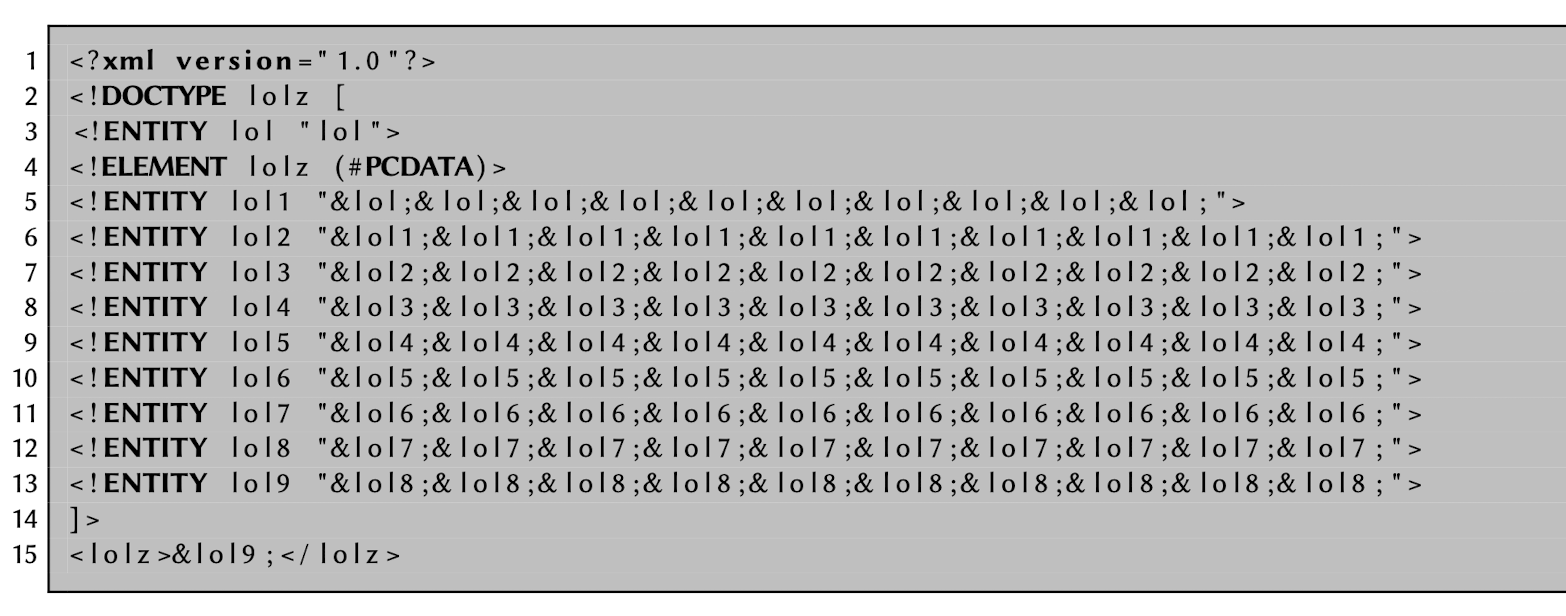
\includegraphics[width=12cm]{img/13_bi_lau.png}
\end{center}



\paragraph{Reflektor-Attacken}
Angreifer sendet Daten an einen oder mehrere Empfänger und diese generieren Verkehr, der an das anzugreifende Ziel gesendet wird. Somit \emph{1)} verbergen sie die wahren Täter und \emph{2)} wird die Bandbreite der Attacke erhöht.\\

Smurf-Attake: Ping-Paket wird mit gefälschter Absender-Adresse an eine Broadcast-Addresse eines Netzwerkes gesendet. Schlecht konfigurierte Clients geben darauf Antwort, indem sie ein Paket an den vermeintlichen Absender (eigentliches Ziel) senden


\paragraph{Drive-By-Infektionen}
Dateien werden "unbeabsichtigt" auf einen Client heruntergeladen. Je nach Ort und Ausgestaltung werden diese Programme ausgeführt und setzen sich auf dem Client fest; Webbrowser -- Verbreitung über angepasste Webseiten (e.g. ungepatchtes CMS)


\newpage
\section{Sicherheit beim Endbenutzer}

\subsection{Berufe in IT-Sicherheit}

\paragraph{Datenschutzbeauftragter} -- Ist für die Einhaltung des Datenschutzes in einer Firma verantwortlich; gibt es in öffentlichen Organen und bei grösseren Firmen; überwacht Fluss und Lagerung von personenrelevanten Daten und sorgt für die Einhaltung der gesetzlichen Grundlagen

\paragraph{Chief Information Security Officer (CISO)} -- Verantwortlich für die interne Sicherheit; definiert Schutzziele einer Organisation und identifiziert Schutzwürdige Objekte; sorgt für Definition und Aufbau der Schutzmassnahmen und überwacht deren Umsetzung

\paragraph{Incident-Manager (IT)} -- Problembehandler in grossen Firmen mit starker Ausprägung in der IT

\paragraph{Forensiker} -- Sammelt belegbar Informationen und liefert revisionssichere Fakten für ein juristisches Verfahren

\paragraph{Fraud-Analyst} -- Spezialist für Aufdecken von Unstimmigkeiten auf betrügerischer Basis aufgrund gegebener Daten

\subsection{Sicherheit beim Enduser}
Entscheidungen, welche Endbenutzer treffen können, um die Sicherheit nachhaltig zu beeinflussen:
\begin{itemize}
\item Auto-Logon-Features
\item Gespeicherte Passworte und Auto-Fill-Optionen ohne hinreichenden Schutz
\item Öffnen von potentiell gefährlichen Mails
\item Verbinden von Geräten mit unsicheren Netzwerken (e.g. gratis WLAN)
\item Verbinden von schlecht geschützter Hardware mit dem Firmennetz
\item Schwache Passworte
\item Hohes Risikoverhalten
\end{itemize}



\subsection{Schutzarten von Sicherheitsmerkmalen}
Sicherheitsmerkmale können auf verschiedene Arten geschützt werden. Jeder Schutz hat Vor- und Nachteile. Schutzarten:
\begin{itemize}
\item Ungeschützt -- Auto-Fill bei Webbrowsern
\item Geschützt mit einem einmalig einzugebenden Sicherheits-Token -- Auto-Fill mit Masterpasswort
\item Geschützt mit einem repetitiv einzugebenden Sicherheits-Token -- Passwortdatenbank mit autoclose und Token-Bestätigung
\end{itemize}

\subsection{Kleine Ursache, Grosse Wirkung}







\end{document}





















